\documentclass{beamer}
\usetheme{dianahep}
%%
% The following was originally taken from a presentation by 
% Jim Pivarski (Princeton University)
% https://www.overleaf.com/7414462kswnjkcfbght#/25712329/
% with subsequent modifications here.
%

%
% Choose how your presentation looks.
%
% For more themes, color themes and font themes, see:
% http://deic.uab.es/~iblanes/beamer_gallery/index_by_theme.html
%
\mode<presentation>
{
  \usetheme{default}      % or try Darmstadt, Madrid, Warsaw, ...
  \usecolortheme{default} % or try albatross, beaver, crane, ...
  \usefonttheme{default}  % or try serif, structurebold, ...
  \setbeamertemplate{navigation symbols}{}
  \setbeamertemplate{caption}[numbered]
  \setbeamertemplate{footline}[page number]
  \setbeamercolor{frametitle}{fg=white}
  \setbeamercolor{footline}{fg=black}
} 

\usepackage[english]{babel}
\usepackage[utf8x]{inputenc}
\usepackage{tikz}
\usepackage{listings}
\usepackage{courier}

\xdefinecolor{darkblue}{rgb}{0.1,0.1,0.7}
\xdefinecolor{dianablue}{rgb}{0.18,0.24,0.31}
\definecolor{commentgreen}{rgb}{0,0.6,0}
\definecolor{stringmauve}{rgb}{0.58,0,0.82}

\lstset{ %
  backgroundcolor=\color{white},      % choose the background color
  basicstyle=\ttfamily\small,         % size of fonts used for the code
  breaklines=true,                    % automatic line breaking only at whitespace
  captionpos=b,                       % sets the caption-position to bottom
  commentstyle=\color{commentgreen},  % comment style
  escapeinside={\%*}{*)},             % if you want to add LaTeX within your code
  keywordstyle=\color{blue},          % keyword style
  stringstyle=\color{stringmauve},    % string literal style
  showstringspaces=false,
  showlines=true
}

\lstdefinelanguage{scala}{
  morekeywords={abstract,case,catch,class,def,%
    do,else,extends,false,final,finally,%
    for,if,implicit,import,match,mixin,%
    new,null,object,override,package,%
    private,protected,requires,return,sealed,%
    super,this,throw,trait,true,try,%
    type,val,var,while,with,yield},
  otherkeywords={=>,<-,<\%,<:,>:,\#,@},
  sensitive=true,
  morecomment=[l]{//},
  morecomment=[n]{/*}{*/},
  morestring=[b]",
  morestring=[b]',
  morestring=[b]"""
}




% Title:
% Building the Research Software Cyberinfrastructure for Particle Physics
%
% Abstract:
% If you visit a laboratory hosting particle physics experiments,
% such as Fermi National Accelerator Laboratory or the European Laboratory for
% Particle Physics (CERN), you will likely be introduced to the
% basic infrastructure of these labs: large particle detectors, even larger
% particle accelerators and perhaps racks of computers in the computer
% center. In practice, another invisible part of the infrastructure ties
% together many of these labs and often outlasts the physically visible
% infrastructure: the software used to manage, process and analyze the
% data produced by the experiments. In this talk I will give an overview
% of the nature and evolution of this research software infrastructure.
% I will also discuss current efforts to build national and international
% collaborations between physicists, computer scientists and industry
% to do the R&D needed for the software for the next generation of particle
% physics experiments.
%
% Bio:
% Peter Elmer is an experimental particle physicist whose area of
% expertise is developing the software and computing systems needed
% to operate and produce scientific results from high energy physics
% experiments. His current research focuses on the Compact Muon
% Solenoid (CMS) experiment at the Large Hadron Collider (LHC) at the
% European Laboratory for Particle Physics (CERN). In the past he has
% worked on the ALEPH experiment at CERN and the BaBar experiment at
% the Stanford Linear Accelerator Center (SLAC). He received a Ph.D.
% in Experimental High Energy Physics from the University of
% Wisconsin - Madison and is a staff researcher at Princeton University
% since 2001.

% https://events.wayne.edu/2017/06/22/scicomp-wayne-seminar-building-the-research-software-cyberinfrastructure-fo-72051/

\title{Building the Research Software Cyberinfrastructure for Particle Physics}
\author{Peter Elmer \\ Princeton University}
\date{22 June, 2017} 

\begin{document}

%\logo{\pgfputat{\pgfxy(0.11, 8)}{\pgfbox[right,base]{\tikz{\filldraw[fill=dianablue, draw=none] (0 cm, 0 cm) rectangle (50 cm, 1 cm);}}}\pgfputat{\pgfxy(0.11, -0.6)}{\pgfbox[right,base]{\tikz{\filldraw[fill=dianablue, draw=none] (0 cm, 0 cm) rectangle (50 cm, 1 cm);}
\includegraphics[height=0.99 cm]{images/diana-hep-logo.png}\tikz{\filldraw[fill=dianablue, draw=none] (0 cm, 0 cm) rectangle (4.9 cm, 1 cm);}}}}




\begin{frame}
  \titlepage
\end{frame}

%\logo{\pgfputat{\pgfxy(0.11, 8)}{\pgfbox[right,base]{\tikz{\filldraw[fill=dianablue, draw=none] (0 cm, 0 cm) rectangle (50 cm, 1 cm);}
\includegraphics[height=1 cm]{images/diana-hep-logo.png}}}}




% Uncomment these lines for an automatically generated outline.
%\begin{frame}{Outline}
%  \tableofcontents
%\end{frame}

\begin{frame}
\frametitle{My background}

\begin{itemize}
\item Experimental Particle Physicist (High Energy Physics, HEP)
\item I primarily work on building the software and computing systems in large particle physics experiments
\item Research Staff with Princeton, based in Geneva, Switzerland
\end{itemize}

\begin{figure}[htbp]
\begin{center}
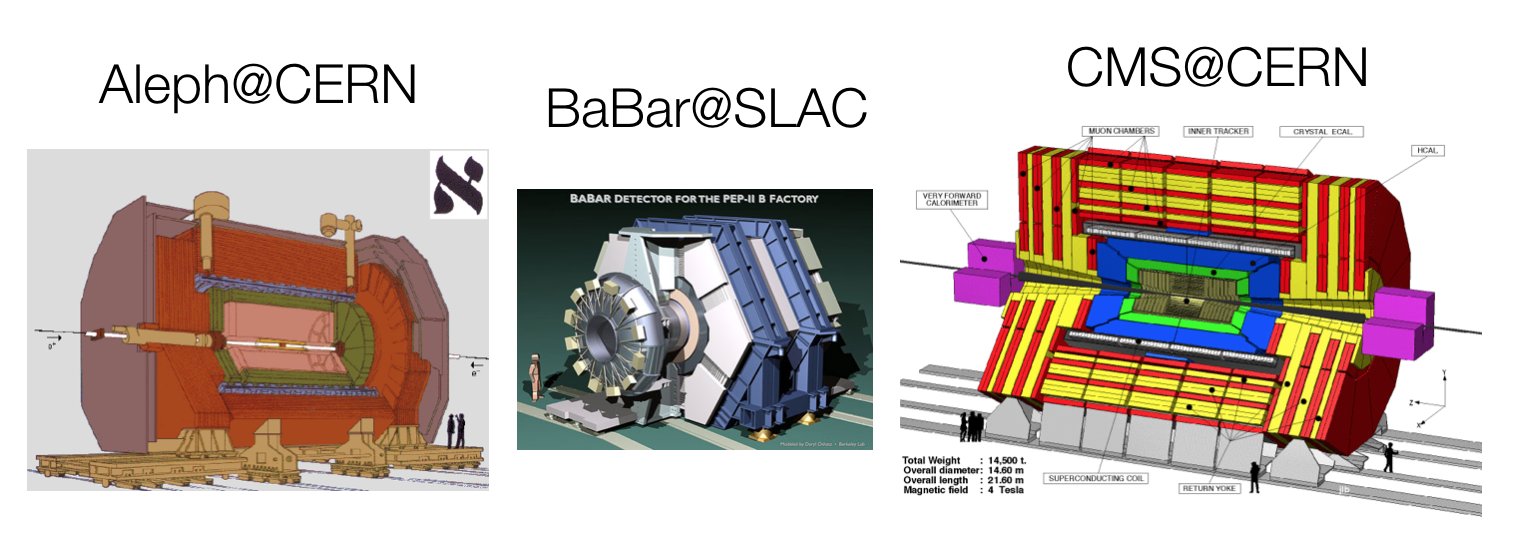
\includegraphics[width=0.9\textwidth]{images/aleph-babar-cms-experiments.png}
%\caption{}
%\label{fig:example2}
\end{center}
\end{figure}

%\small{Example Text}

\end{frame}




%\begin{frame}
\frametitle{Large Hadron Collider}

\begin{itemize}
\item What kind of research are you doing with data?
\item Any privacy issues with the data? Reliability?
\item What kind of data and what size/features ("by the numbers")
\item What institutions are involved in collaboration? And how do they share data?
\item Data created by the team or acquired from elsewhere?
\item What storage/compute platforms are you currently using (private, local shared, public)?
\item How is data, computation/storage, and results shared among PIs/institutions?
\item What would best accelerate your research? (tools, training, public resources)
\end{itemize}

\end{frame}



\begin{frame}
\frametitle{LHC Grand Challenge Research Questions}

The goal of HEP (and the LHC) is to understand the fundamental building blocks of nature, and their interactions. The potential of the LHC has been demonstrated in its first years with the discovery of the Higgs Boson. \\
\vskip 0.15in
\begin{figure}[htbp]
\begin{center}
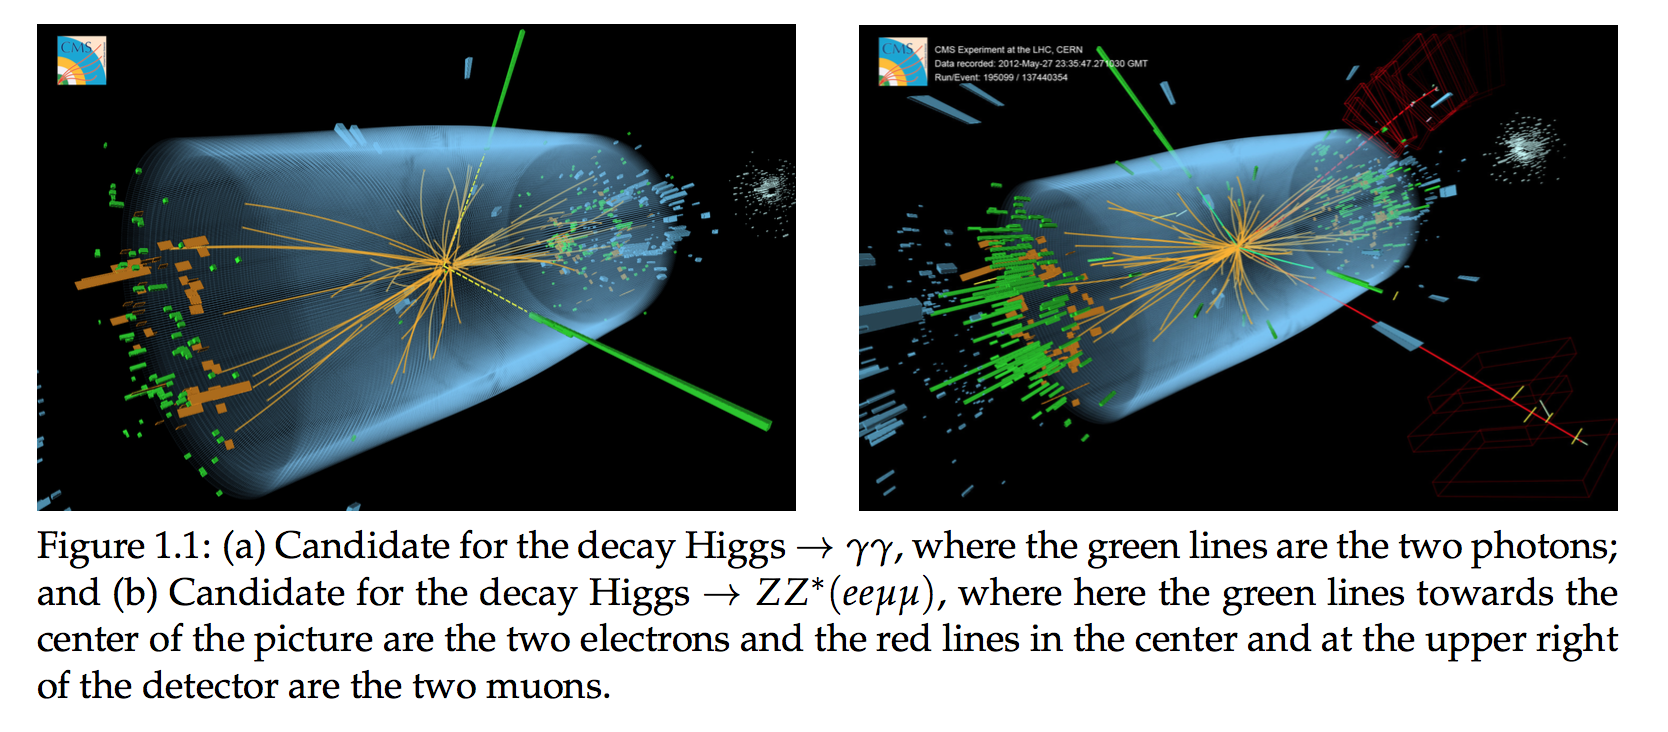
\includegraphics[width=1.0\textwidth]{images/cms-higgs-events.png}
%\caption{}
%\label{fig:example2}
\end{center}
\end{figure}

\end{frame}



\begin{frame}
\frametitle{LHC Grand Challenge Research Questions}

Many fundamental questions remain, however, including: Why does nature express the symmetries embodied in the Standard Model, and not other equally elegant symmetries? Why are there (only) three generations of basic building blocks of matter? Why are the masses of these building blocks so different from each other, both within a generation and between generations? What is the dark matter which pervades the Universe? Why is matter so dominant over antimatter in the Universe? Does space-time have additional symmetries or extend beyond the 3+1 dimensions of which we know? What mechanism stabilizes the Higgs mass from large quantum corrections at high energy? Are neutrinos their own anti-particles? Can gravity and quantum mechanics be described in a consistent theoretical framework?

\end{frame}



\begin{frame}
\frametitle{Large Hadron Collider (LHC)}

\begin{columns}[T] % align columns

\begin{column}{.50\textwidth}
\begin{itemize}
\item A 27km ring of superconducting magnets in a circular tunnel $\sim$100m under the Swiss-French border near Geneva
\item The world's highest energy proton-proton collider (replaced Tevatron at Fermilab for this kind of physics)
\end{itemize}
\end{column}%


\begin{column}{.50\textwidth}
\begin{figure}[htbp]
\begin{center}
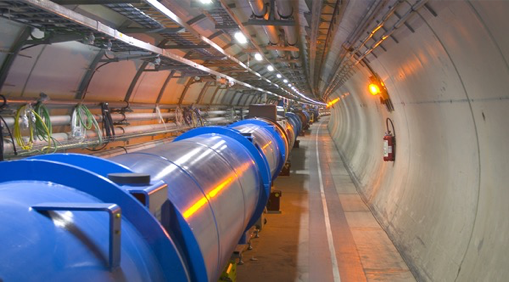
\includegraphics[width=0.9\textwidth]{images/lhc-tunnel.png}
%\caption{}
%\label{fig:example2}
\end{center}
\end{figure}
\end{column}%

\end{columns}

\begin{itemize}
\item From an initial project idea more than 30 years ago, it was built in the existing tunnel designed for previous LEP accelerator
\item The experiments began planning 25 years ago
\end{itemize}


%\small{Example Text}

\end{frame}



\begin{frame}
\frametitle{Large Hadron Collider (LHC) and Experiments}

\begin{figure}[htbp]
\begin{center}
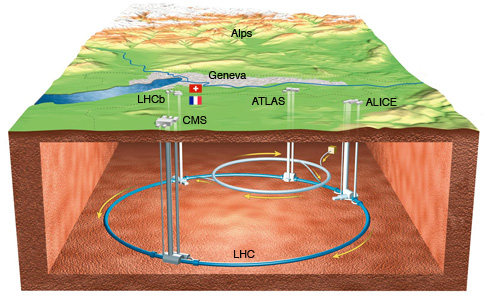
\includegraphics[width=0.8\textwidth]{images/CERNMap.jpg}
%\caption{}
%\label{fig:example2}
\end{center}
\end{figure}

\small{Two very large experiments (Atlas, CMS) with 3500+ people, and two large experiments (Alice, LHCb) with 500+ people}

\end{frame}



\begin{frame}
\frametitle{Needle in a haystack problems}

\begin{columns}[T] % align columns

\begin{column}{.50\textwidth}
\begin{figure}[htbp]
\begin{center}
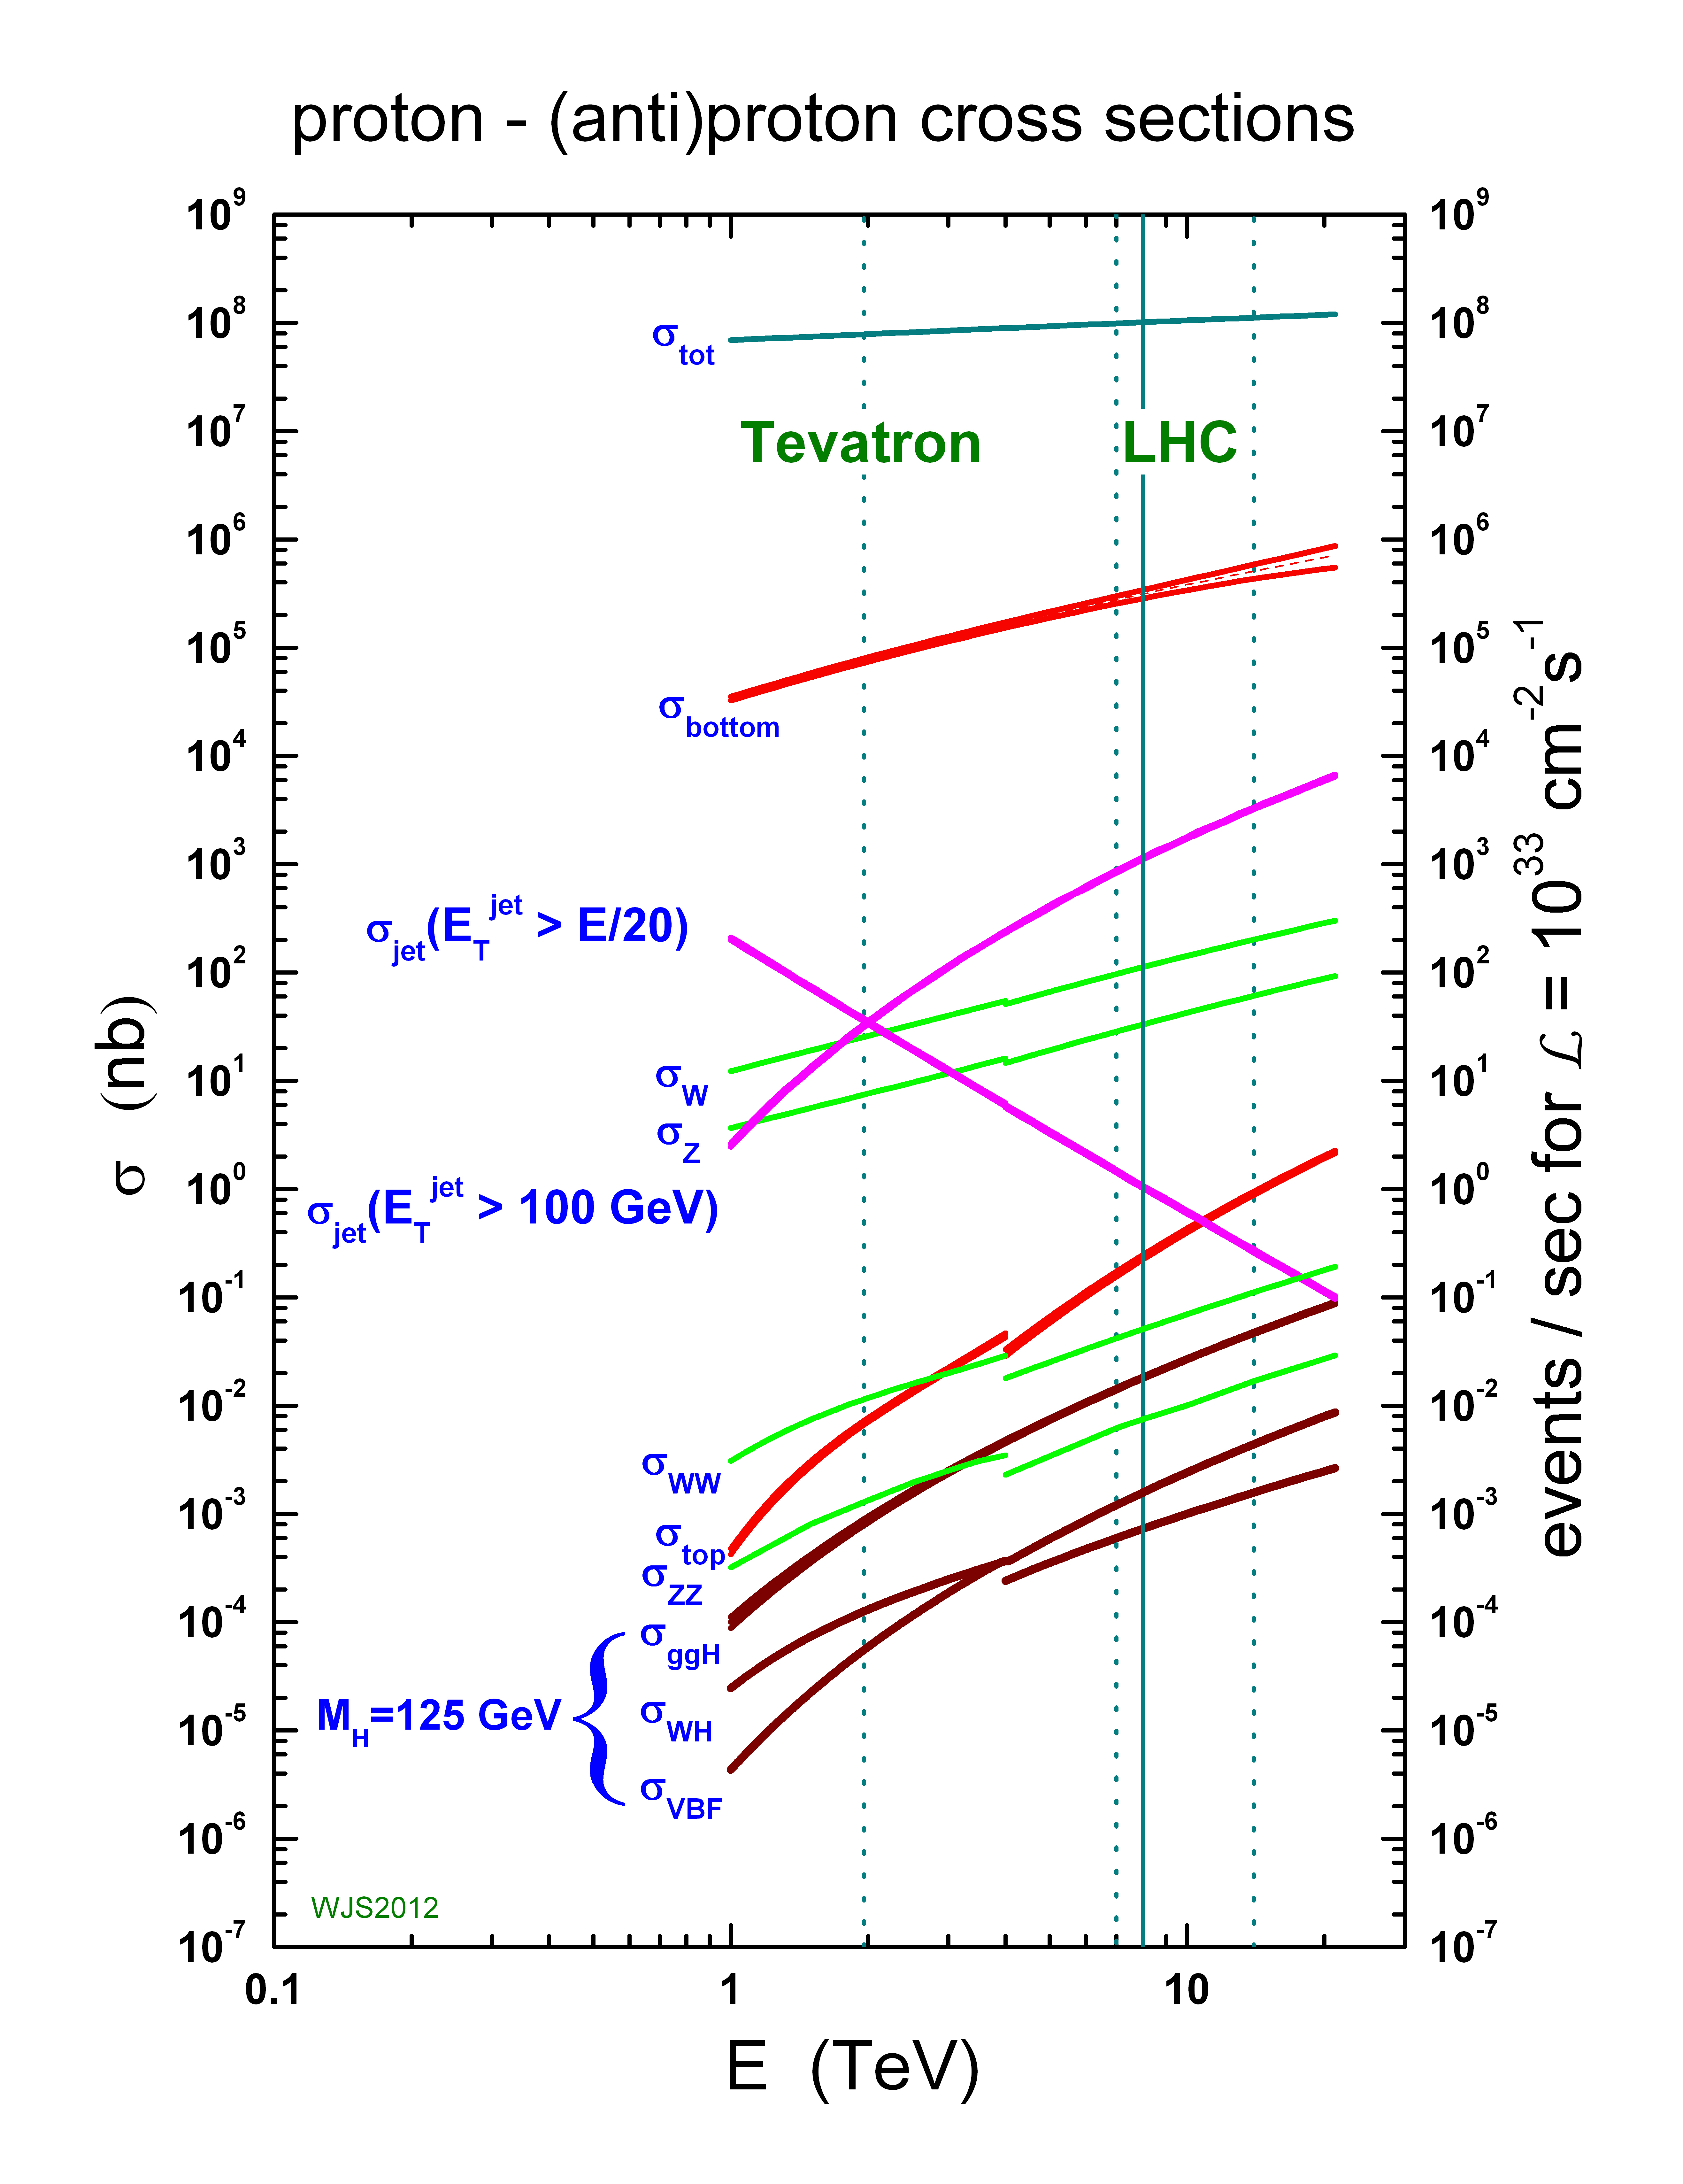
\includegraphics[width=0.9\textwidth]{images/crosssections2013.jpeg}
%\caption{}
%\label{fig:example2}
\end{center}
\end{figure}
\end{column}%

\begin{column}{.50\textwidth}
\vskip 0.5in
\begin{itemize}
\item Show is the production rates for various processes versus center-of-mass energy of collisions
\item Orders of magnitude difference between signal and background
\item Colliders have two ``knobs'': the energy and the ``luminosity'' (intensity) of collisions
\end{itemize}
\end{column}%




\end{columns}

%\small{Example Text}

\end{frame}




\begin{frame}
\frametitle{CMS Detector}

\begin{figure}[htbp]
\begin{center}
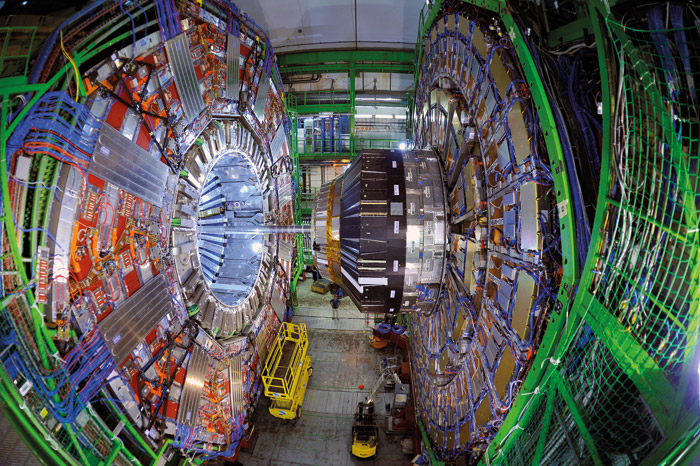
\includegraphics[width=0.8\textwidth]{images/CMS_CC204_05_13.jpeg}
%\caption{}
%\label{fig:example2}
\end{center}
\end{figure}

%\small{Example Text}

\end{frame}



\begin{frame}
\frametitle{CMS Detector}

\begin{figure}[htbp]
\begin{center}
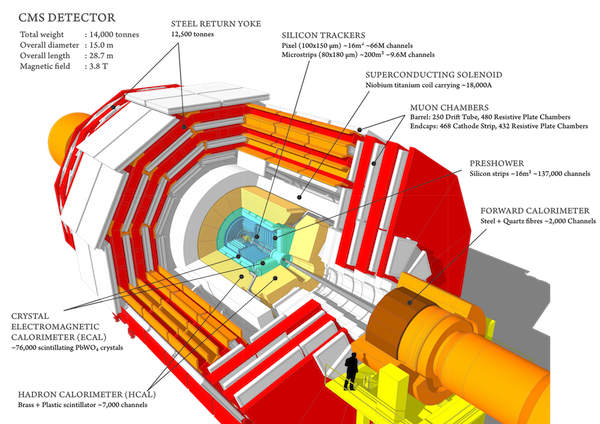
\includegraphics[width=0.8\textwidth]{images/cms_120918_03_small.png}
%\caption{}
%\label{fig:example2}
\end{center}
\end{figure}

%\small{Example Text}

\end{frame}



\begin{frame}
\frametitle{Example slice of detector}

\begin{figure}[htbp]
\begin{center}
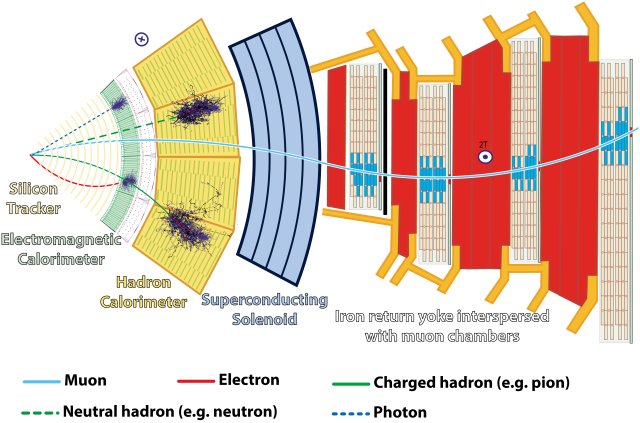
\includegraphics[width=0.9\textwidth]{images/CMSslice_whiteBackground.png}
%\caption{}
%\label{fig:example2}
\end{center}
\end{figure}

%\small{Example Text}

\end{frame}




\begin{frame}
\frametitle{Worldwide LCG Computing Grid}

\begin{figure}[htbp]
\begin{center}
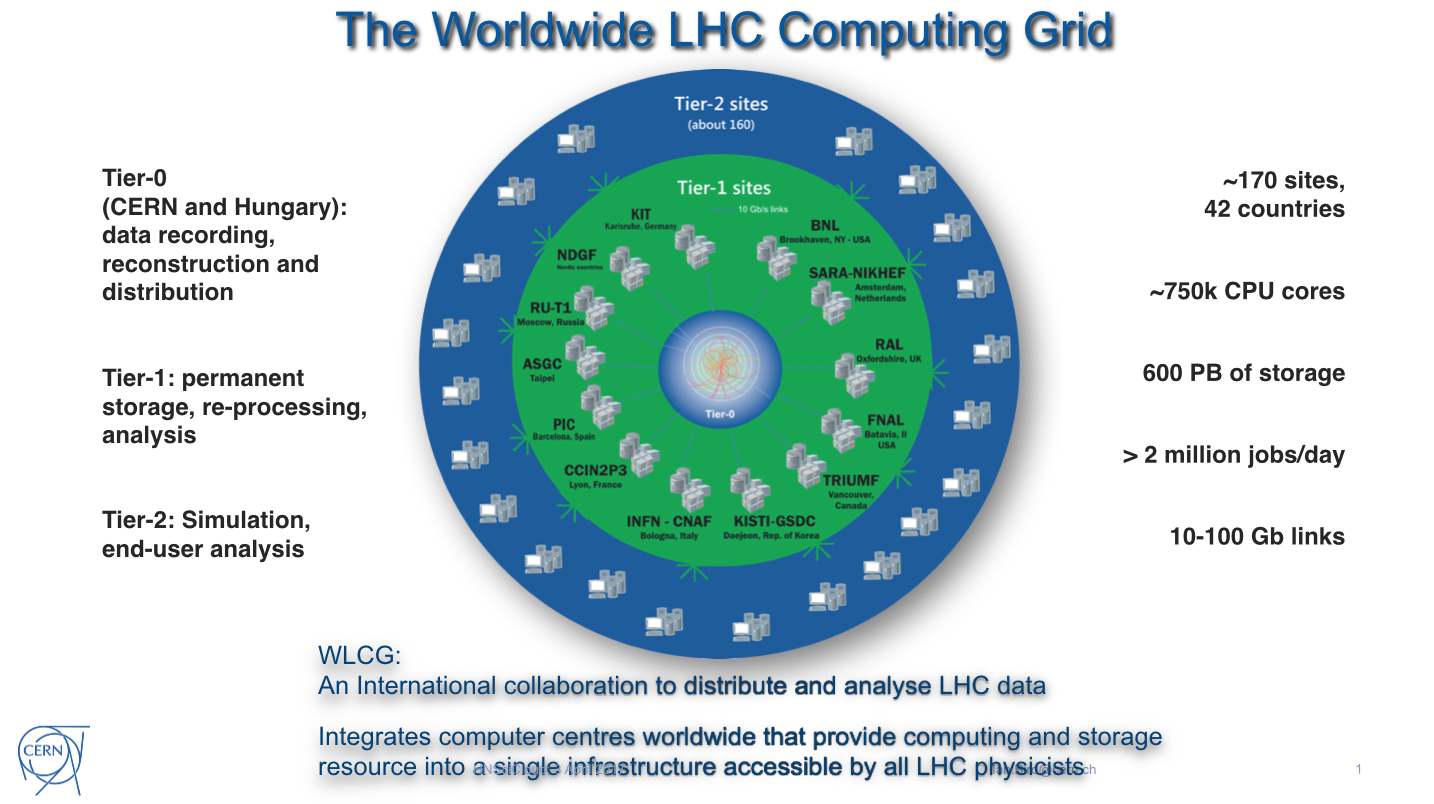
\includegraphics[width=1.0\textwidth]{images/WLCG-2017.png}
%\caption{}
%\label{fig:example2}
\end{center}
\end{figure}
\end{frame}




\begin{frame}
\frametitle{Cyberinfrastructure?}

\begin{columns}[T] % align columns

\begin{column}{.70\textwidth}
\begin{figure}[htbp]
\begin{center}
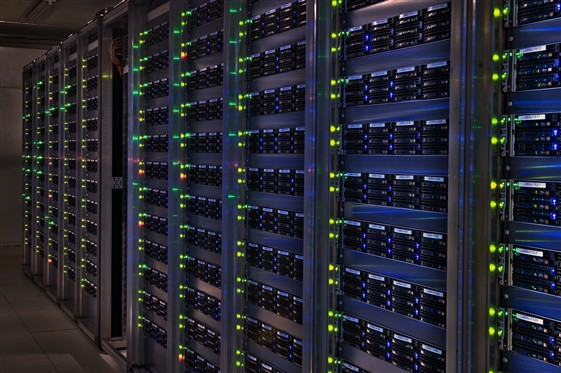
\includegraphics[width=0.9\textwidth]{images/1008289_02-A5-at-72-dpi.jpg}
%\caption{}
%\label{fig:example2}
\end{center}
\end{figure}
\end{column}%

\begin{column}{.30\textwidth}
\begin{figure}[htbp]
\begin{center}
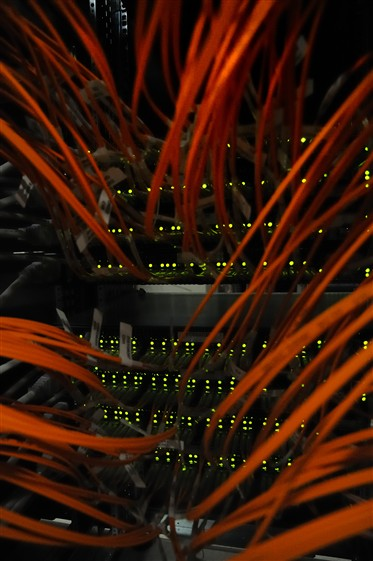
\includegraphics[width=0.93\textwidth]{images/1008291_03-A5-at-72-dpi.jpg}
%\caption{}
%\label{fig:example2}
\end{center}
\end{figure}
\end{column}%




\end{columns}

%\small{Example Text}

\end{frame}



\begin{frame}
\frametitle{Why Software? Software is {\em the} Cyberinfrastructure}

\begin{figure}[htbp]
\begin{center}
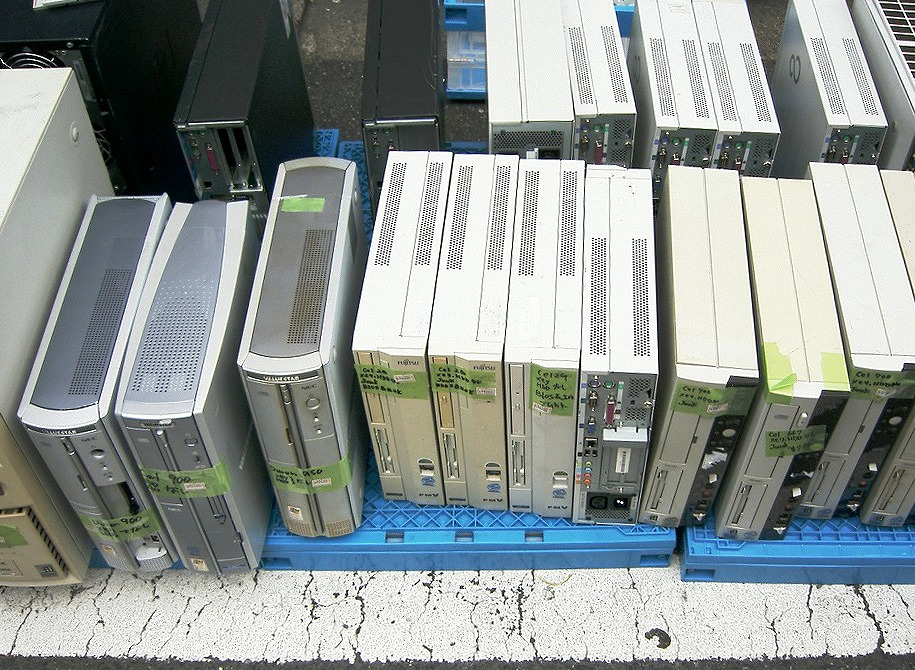
\includegraphics[width=0.7\textwidth]{images/Junk_desktop_personal_computer.jpg}
%\caption{}
%\label{fig:example2}
\end{center}
\end{figure}

\begin{center}
\small{Computer hardware is a consumable. \\ Software is what we keep, and invest in, over time.}
\end{center}

\end{frame}



\begin{frame}
\frametitle{HEP Software Ecosystem}

\begin{figure}[htbp]
\begin{center}
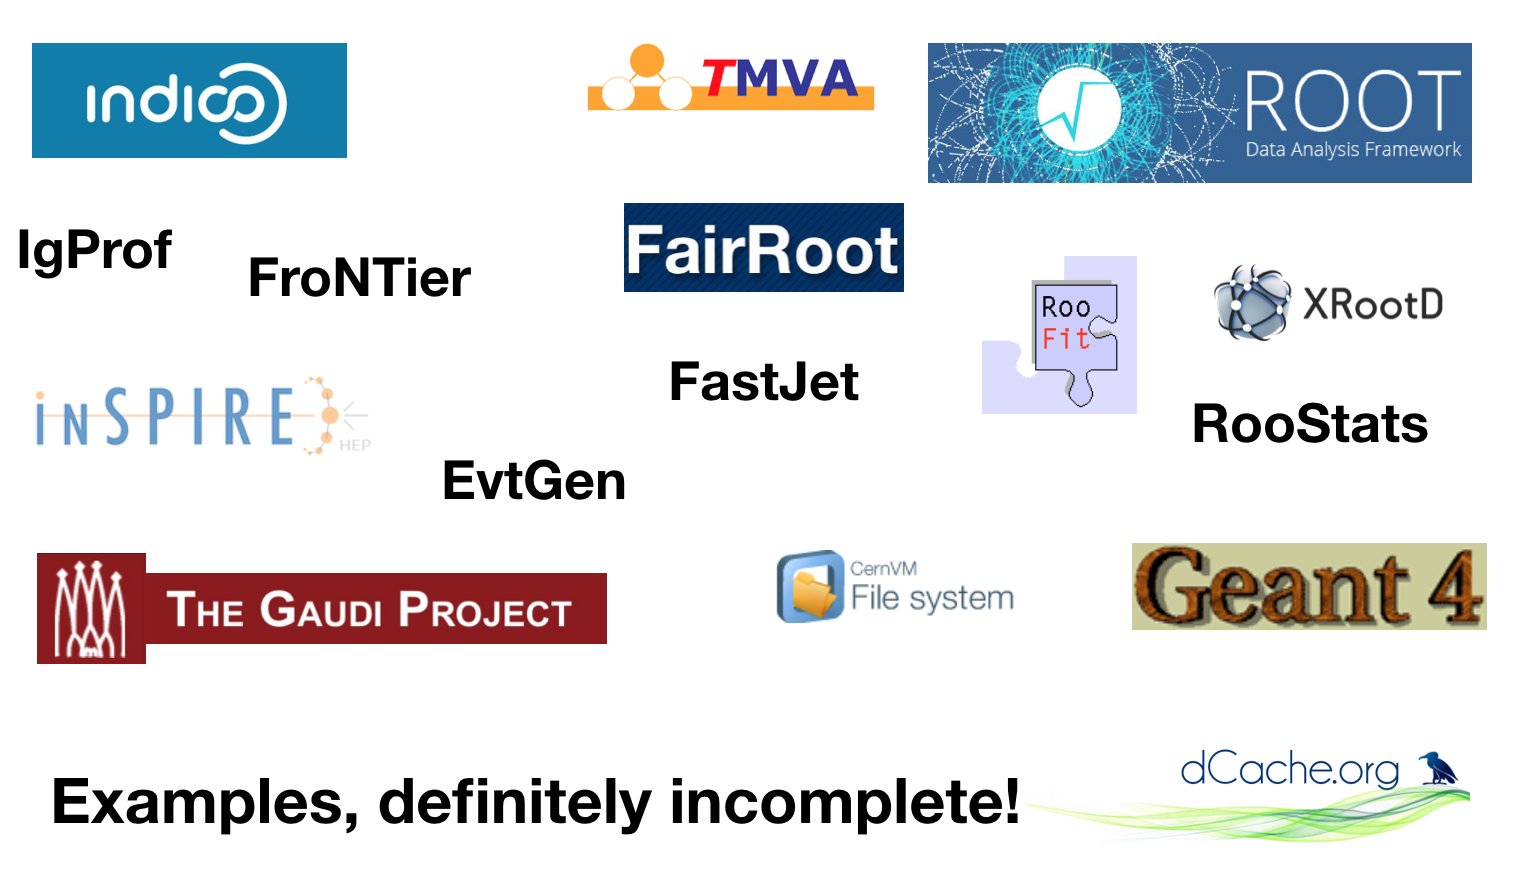
\includegraphics[width=0.85\textwidth]{images/hep-software-ecosystem.png}
%\caption{}
%\label{fig:example2}
\end{center}
\end{figure}
\small{Plus 15-20M Source Lines of Code (SLOC) of “experiment specific” codes, as well as dependencies on non-HEP scientific software.}
\end{frame}




% Activities - algorithmic
\begin{frame}
\frametitle{Charged Particle Tracking Reconstruction}

\begin{figure}[tbp]
\centering
%\includegraphics[width=0.3\linewidth]{PU140-RPhi.png}
%\includegraphics[width=0.3\textwidth]{tmp-RecoTimeLUMI_25_BX_25ns.png}
%\includegraphics[width=0.29\linewidth]{effandfake1_01.png}

%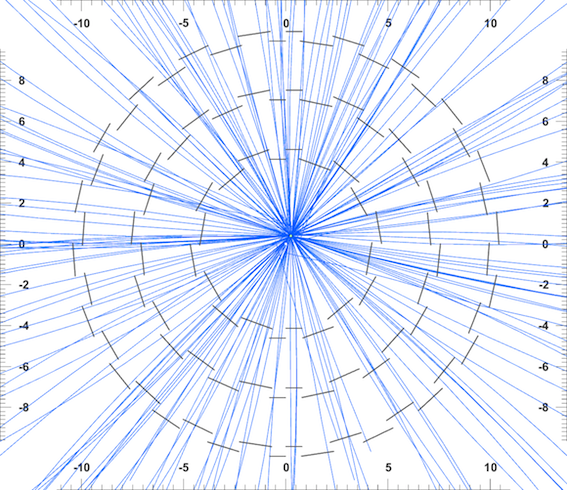
\includegraphics[width=0.32\linewidth]{images/PU50ns_run2_RPhi.png}
%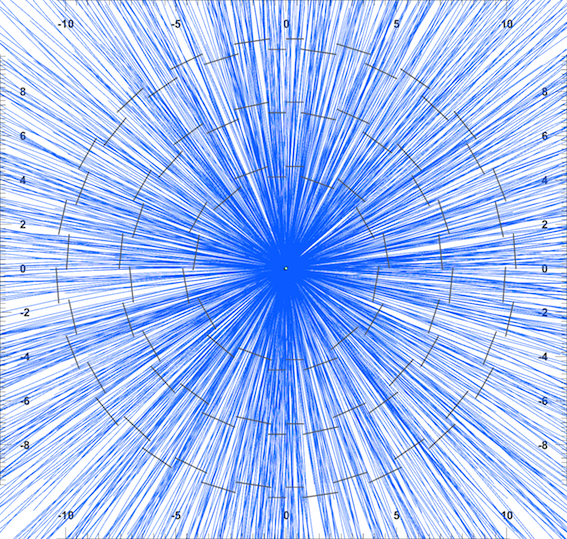
\includegraphics[width=0.3\linewidth]{images/PU140_2023_RPhi.png}
%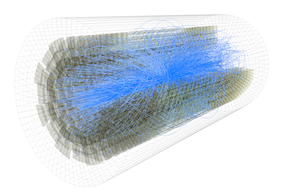
\includegraphics[width=0.3\linewidth]{images/PU140-3D.png}

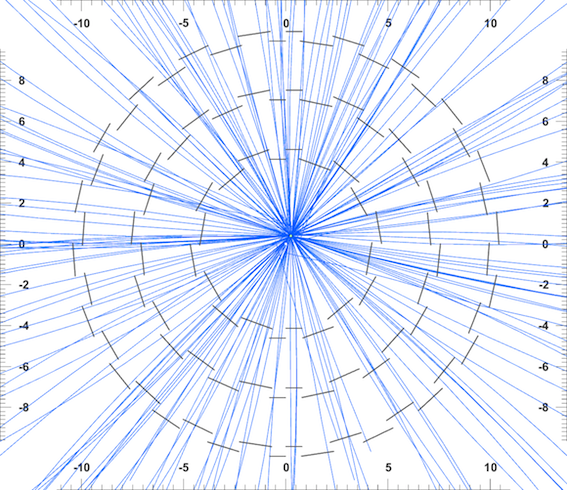
\includegraphics[width=0.5\linewidth]{images/PU50ns_run2_RPhi.png}
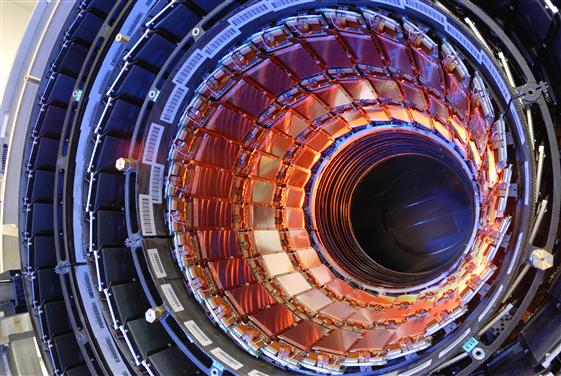
\includegraphics[width=0.5\linewidth]{images/0610026_01-A5-at-72-dpi.jpg}

%\caption{Display of charged particles in transverse plane to beams (r-phi) for
%PU=25 (2013) - left, and PU=140 (2023) - center, and 3D view of
%PU=140 collision - right.}
%\label{fig:PU140-All}
\end{figure}

%\small{Example Text}

\end{frame}



\begin{frame}
\frametitle{Charged Particle Tracking Reconstruction - Event Complexity}

\begin{figure}[tbp]
\centering
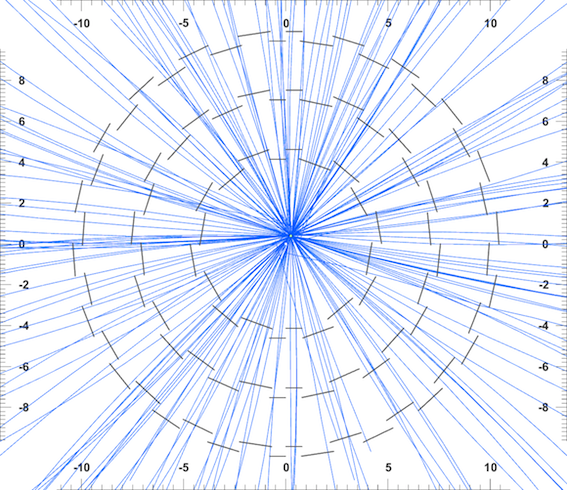
\includegraphics[width=0.32\linewidth]{images/PU50ns_run2_RPhi.png}
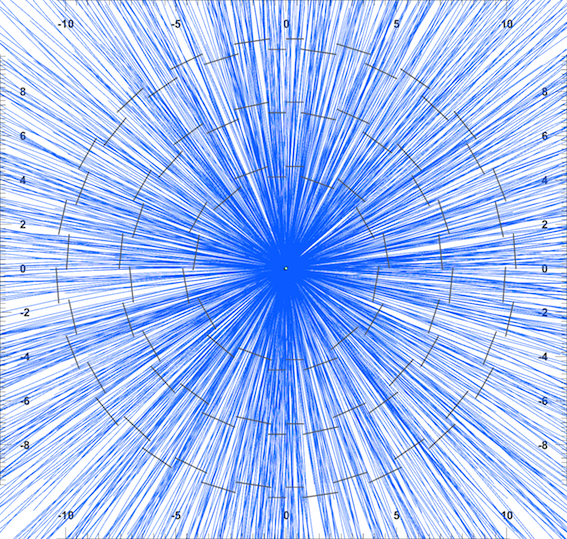
\includegraphics[width=0.3\linewidth]{images/PU140_2023_RPhi.png}
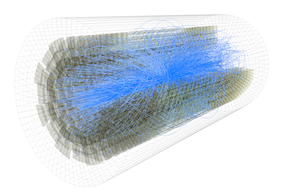
\includegraphics[width=0.3\linewidth]{images/PU140-3D.png}

\caption{Display of charged particles in transverse plane to beams (r-phi) for
PU=25 (2013) - left, and PU=140 (2023) - center, and 3D view of
PU=140 collision - right.}
%\label{fig:PU140-All}
\end{figure}

%\small{Example Text}

\end{frame}



\begin{frame}
\frametitle{CPU and bulk processing capacity}

The vast majority of the CPU needs at the HL-LHC come from pattern recognition algorithms (``reconstruction'' for HEP). This probably a factor of 10 short, assuming we get and can exploit 20\%/year Moore's Law gains.

\begin{figure}[htbp]
\begin{center}
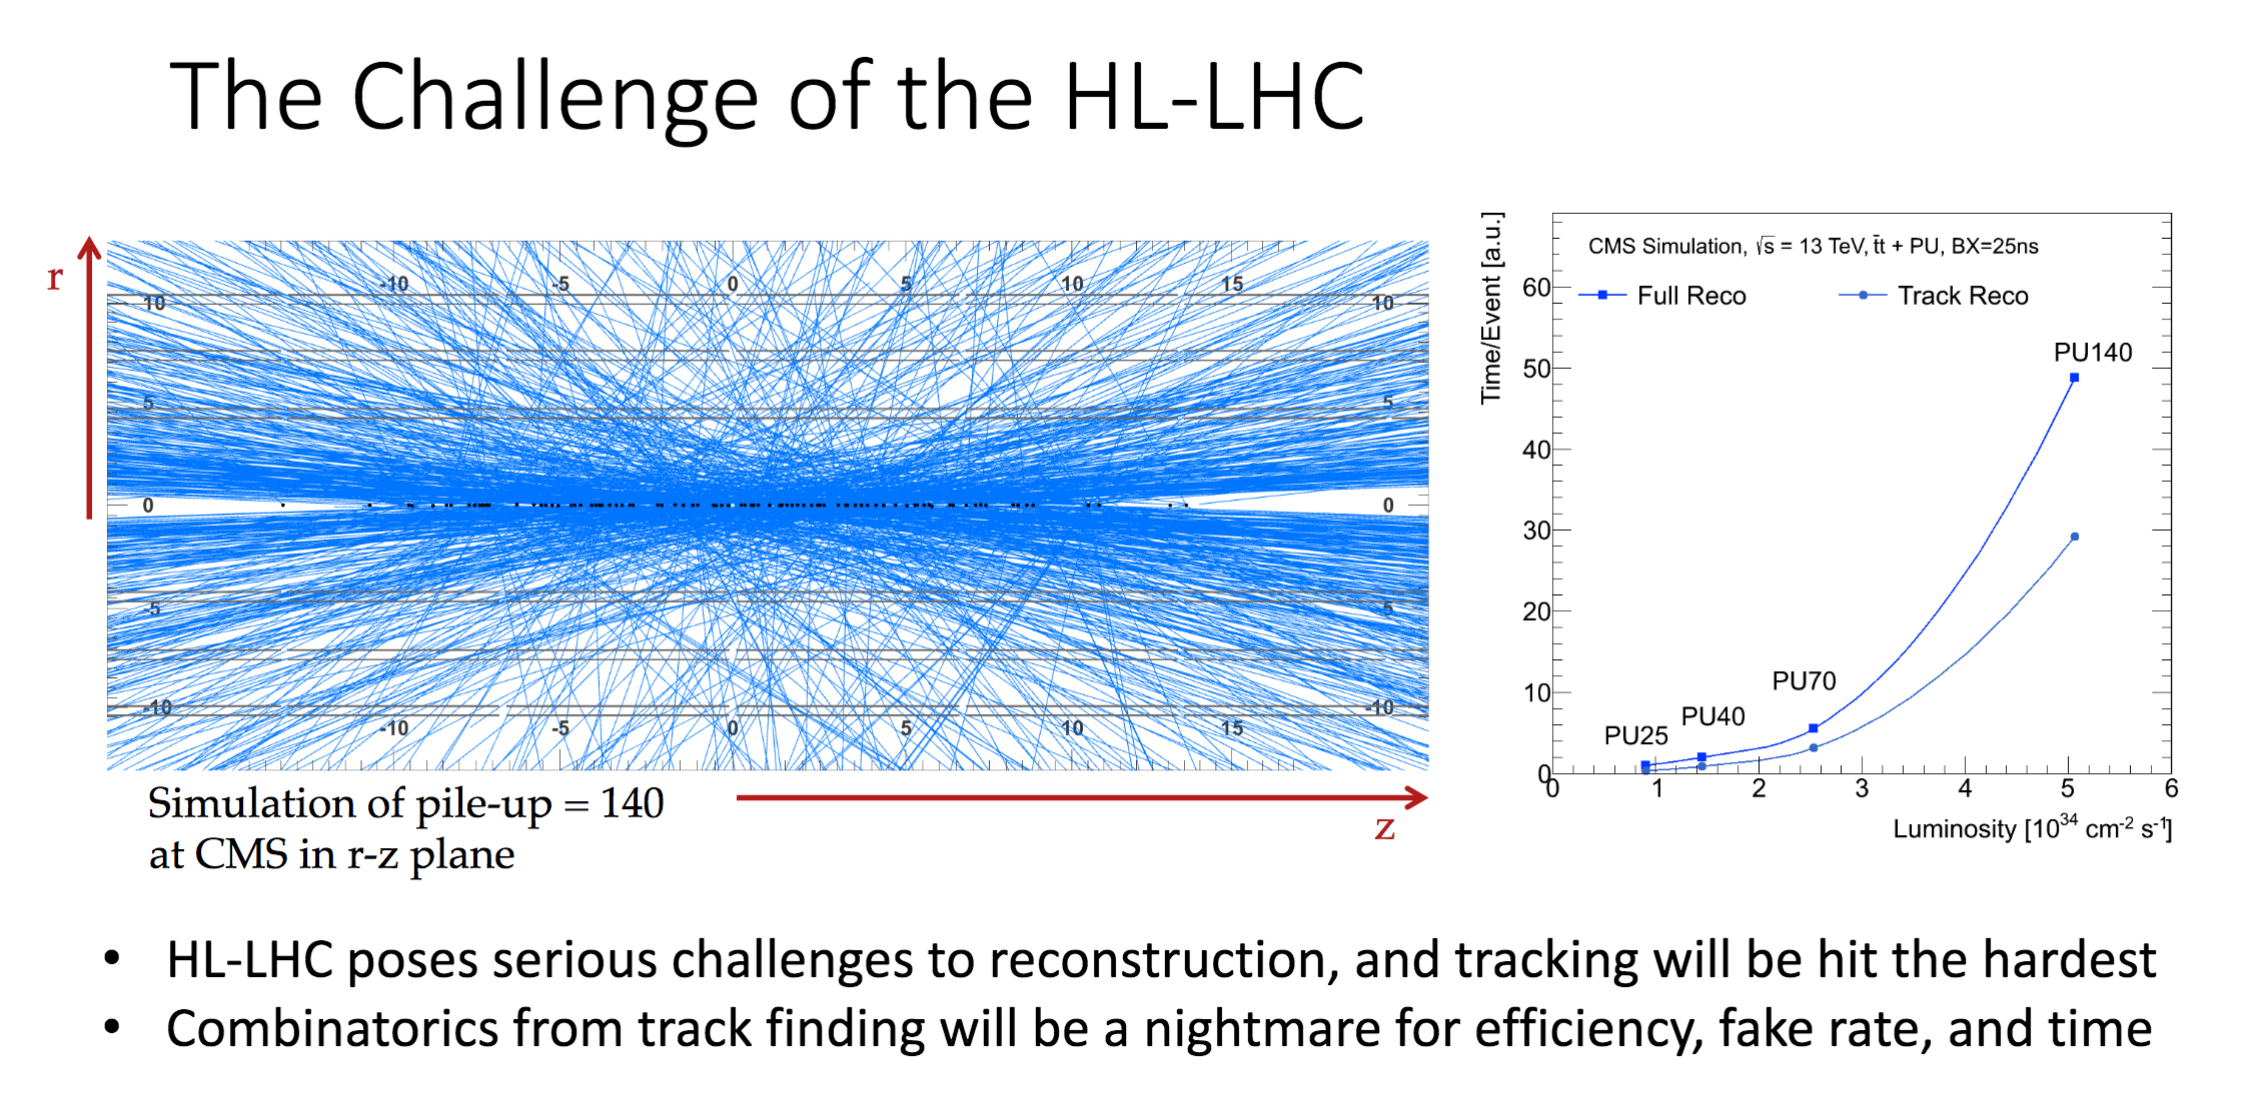
\includegraphics[width=1.0\textwidth]{images/hllhc-reco-tracking.png}
%\caption{}
%\label{fig:example2}
\end{center}
\end{figure}

\end{frame}




\begin{frame}
\frametitle{Higgs Discovery Plot - Use of Monte Carlo Simulation}

\begin{columns}[T] % align columns

\begin{column}{.60\textwidth}
\begin{figure}[htbp]
\begin{center}
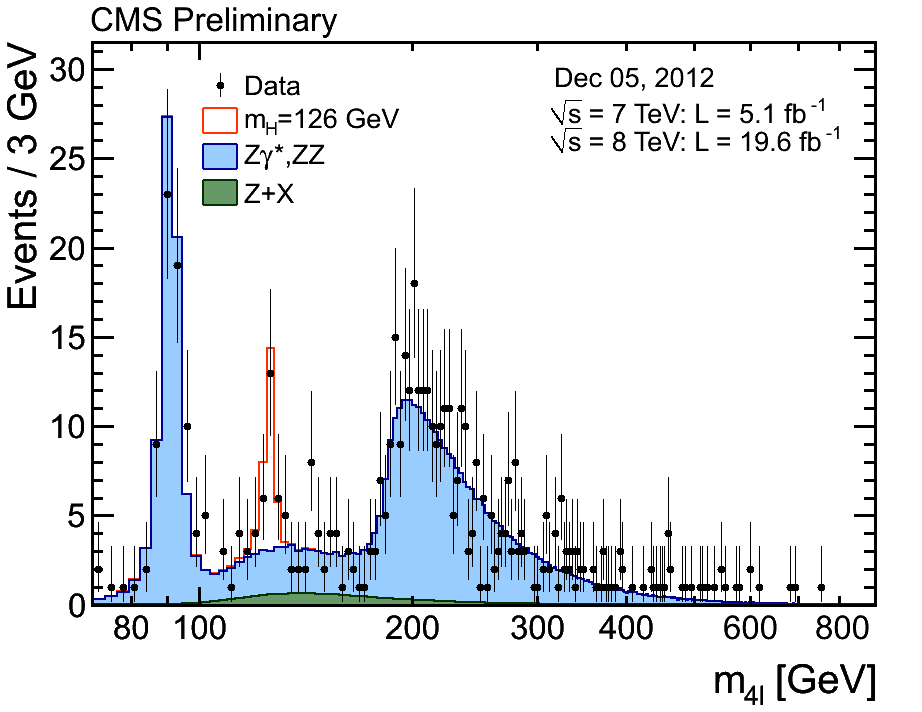
\includegraphics[width=0.95\textwidth]{images/higgs-discovery-plot.png}
%\caption{}
%\label{fig:example2}
\end{center}
\end{figure}
\end{column}%

\begin{column}{.40\textwidth}
\begin{itemize}
\item Detect particle interactions and compare to standard model
\item Black dots (with error bars) are measurements
\item Blue shape: simulation of standard model
\item Red shape: simulation of new theory (in this case the Higgs)
\end{itemize}
\end{column}%

\end{columns}

%\small{Example Text}

\end{frame}



\begin{frame}
\frametitle{Monte Carlo Detector Simulation}

 Contents of the first slide

\end{frame}




\begin{frame}
\frametitle{Software and Computing High Level Workflow}

\begin{figure}[htbp]
\begin{center}
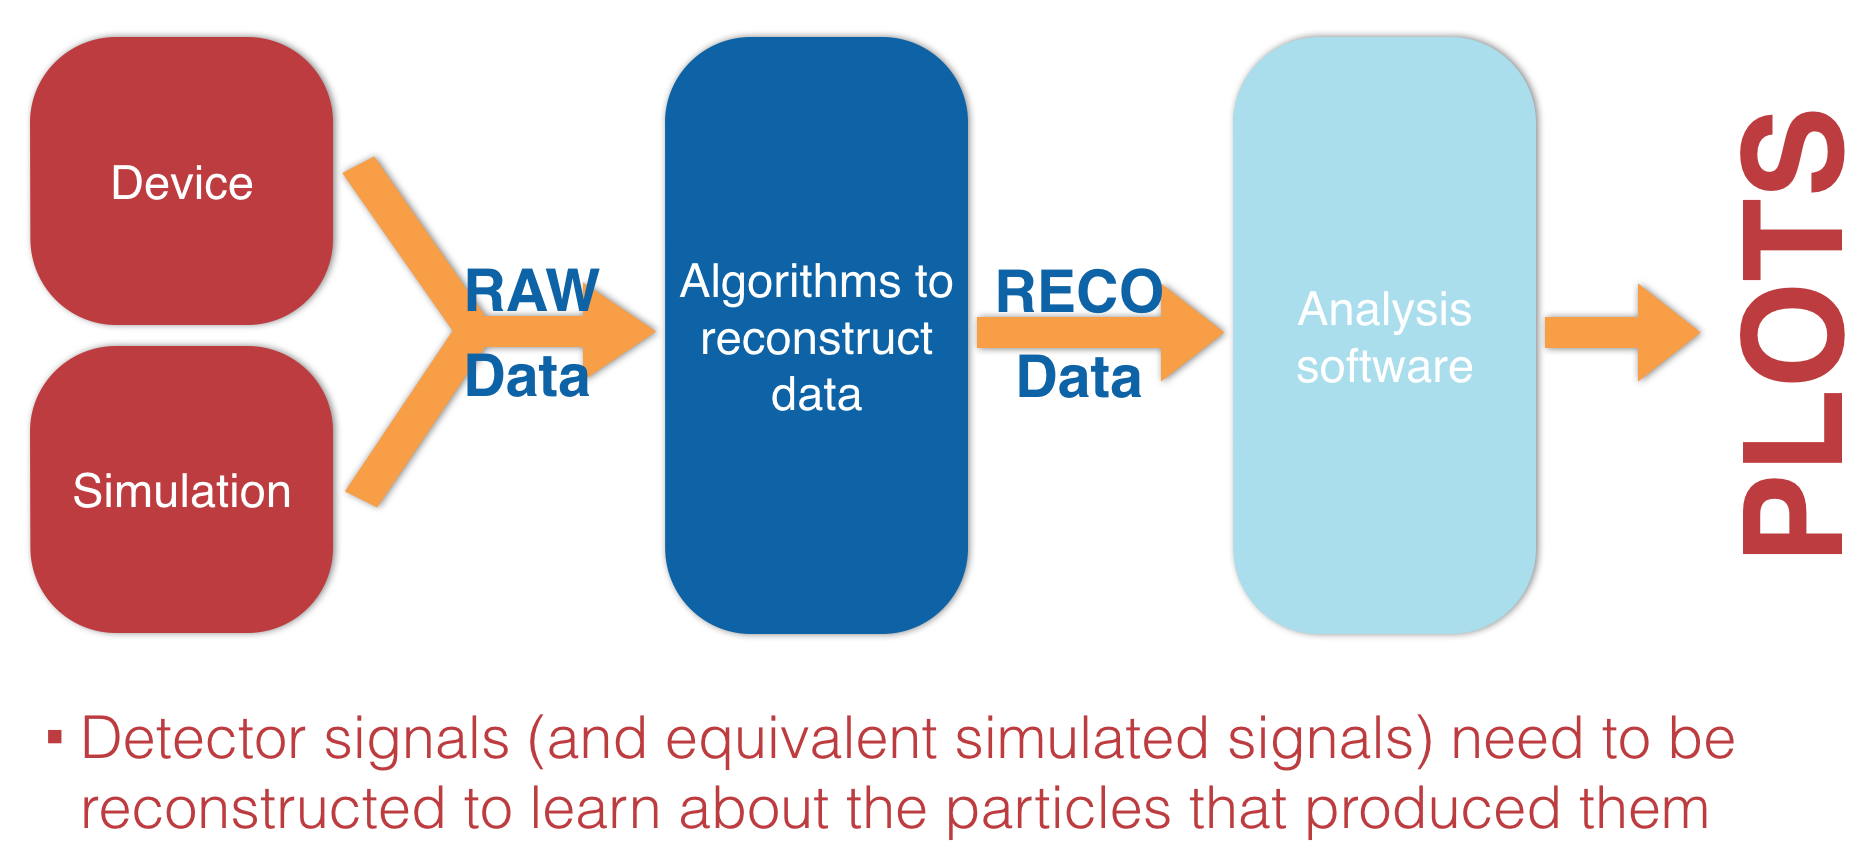
\includegraphics[width=0.7\textwidth]{images/workflow-high-level.png}
%\caption{}
%\label{fig:example2}
\end{center}
\end{figure}

%\small{Example Text}

\end{frame}




\begin{frame}
\frametitle{Analysis Data Reduction - ``Last Mile''}

\begin{figure}[htbp]
\begin{center}
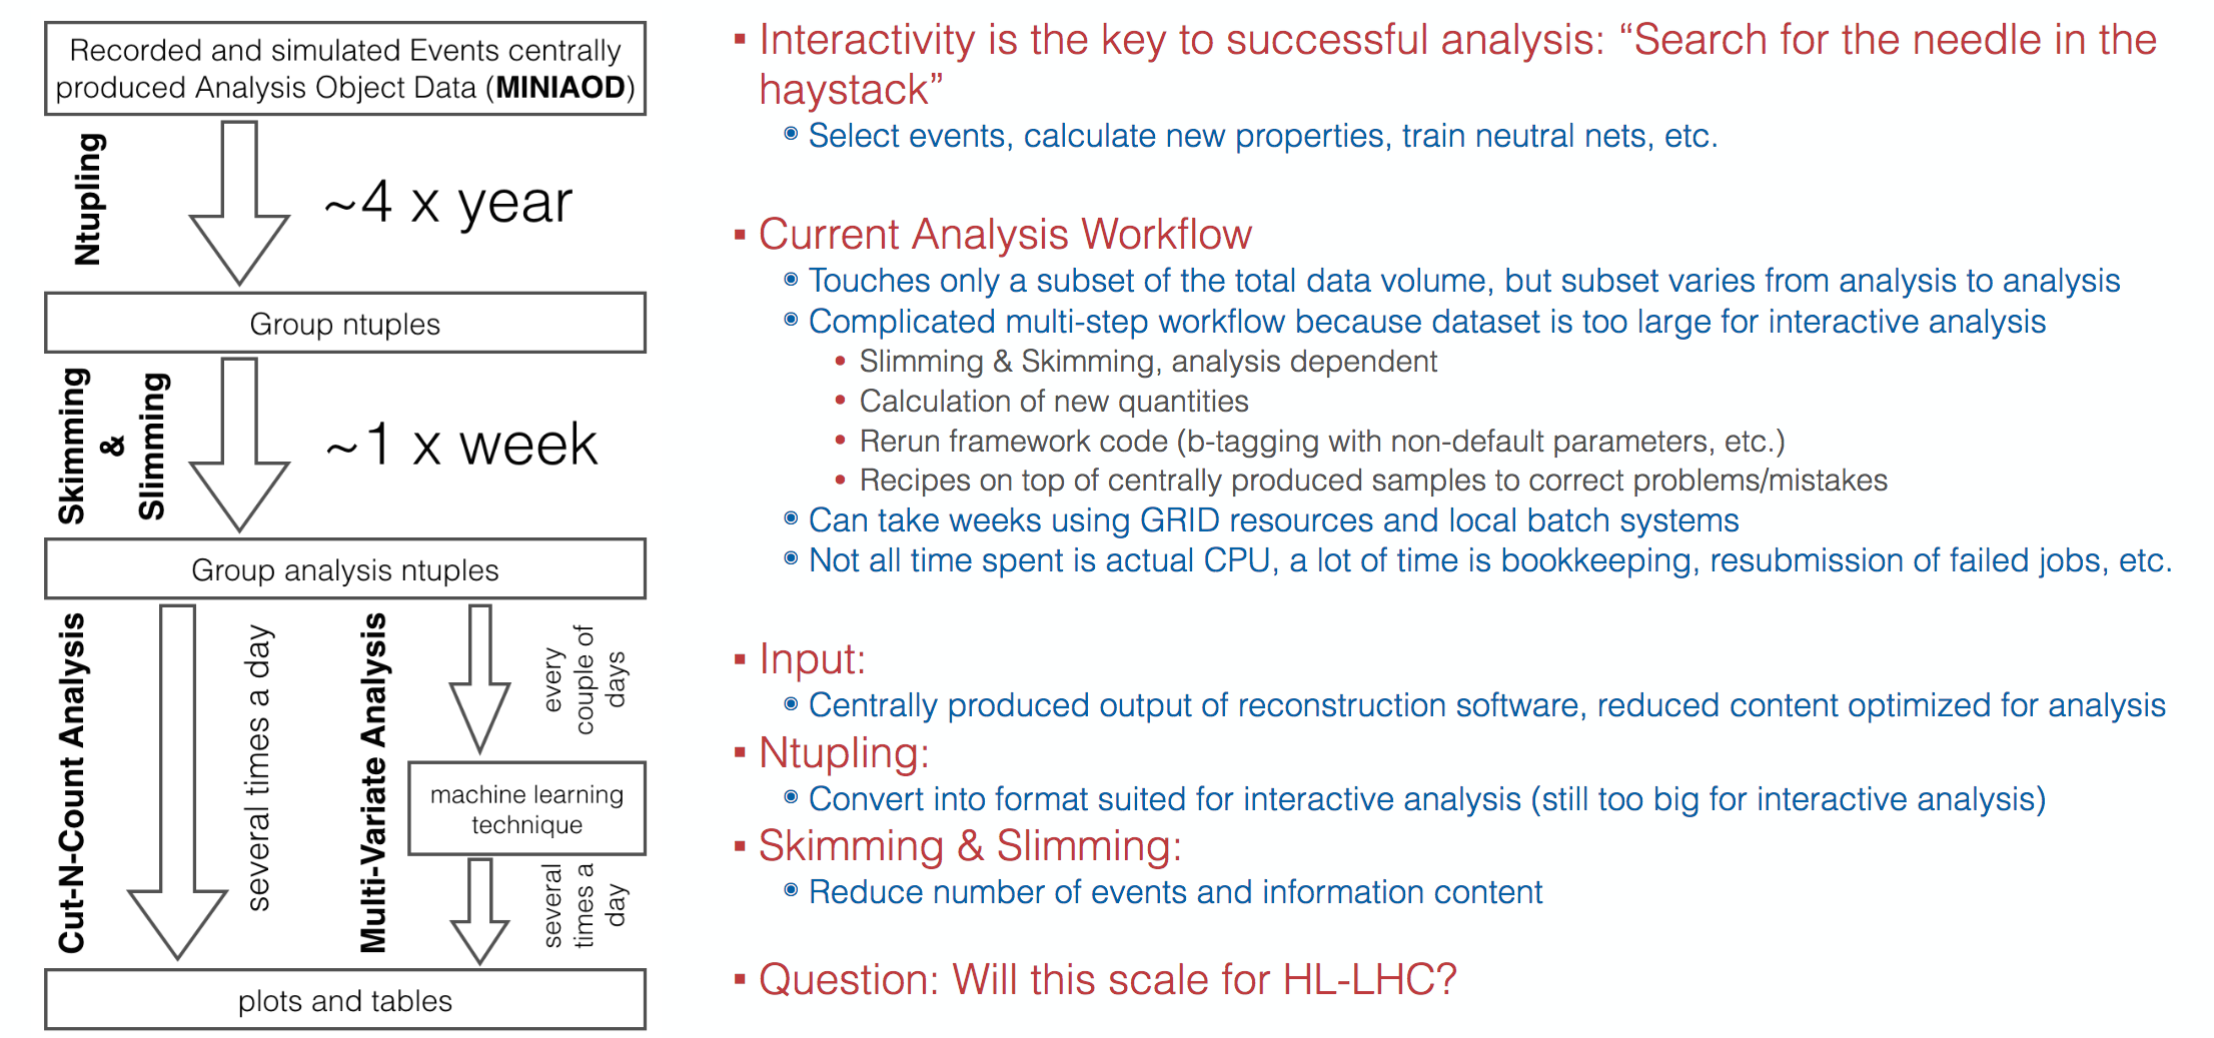
\includegraphics[width=1.0\textwidth]{images/analysis-data-reduction.png}
%\caption{}
%\label{fig:example2}
\end{center}
\end{figure}

\end{frame}



\begin{frame}
\frametitle{ROOT}

 Contents of the first slide

\end{frame}




% Activities - infrastructure
\begin{frame}
\frametitle{Computing Infrastructure for CMS Experiment}

\begin{figure}[htbp]
\begin{center}
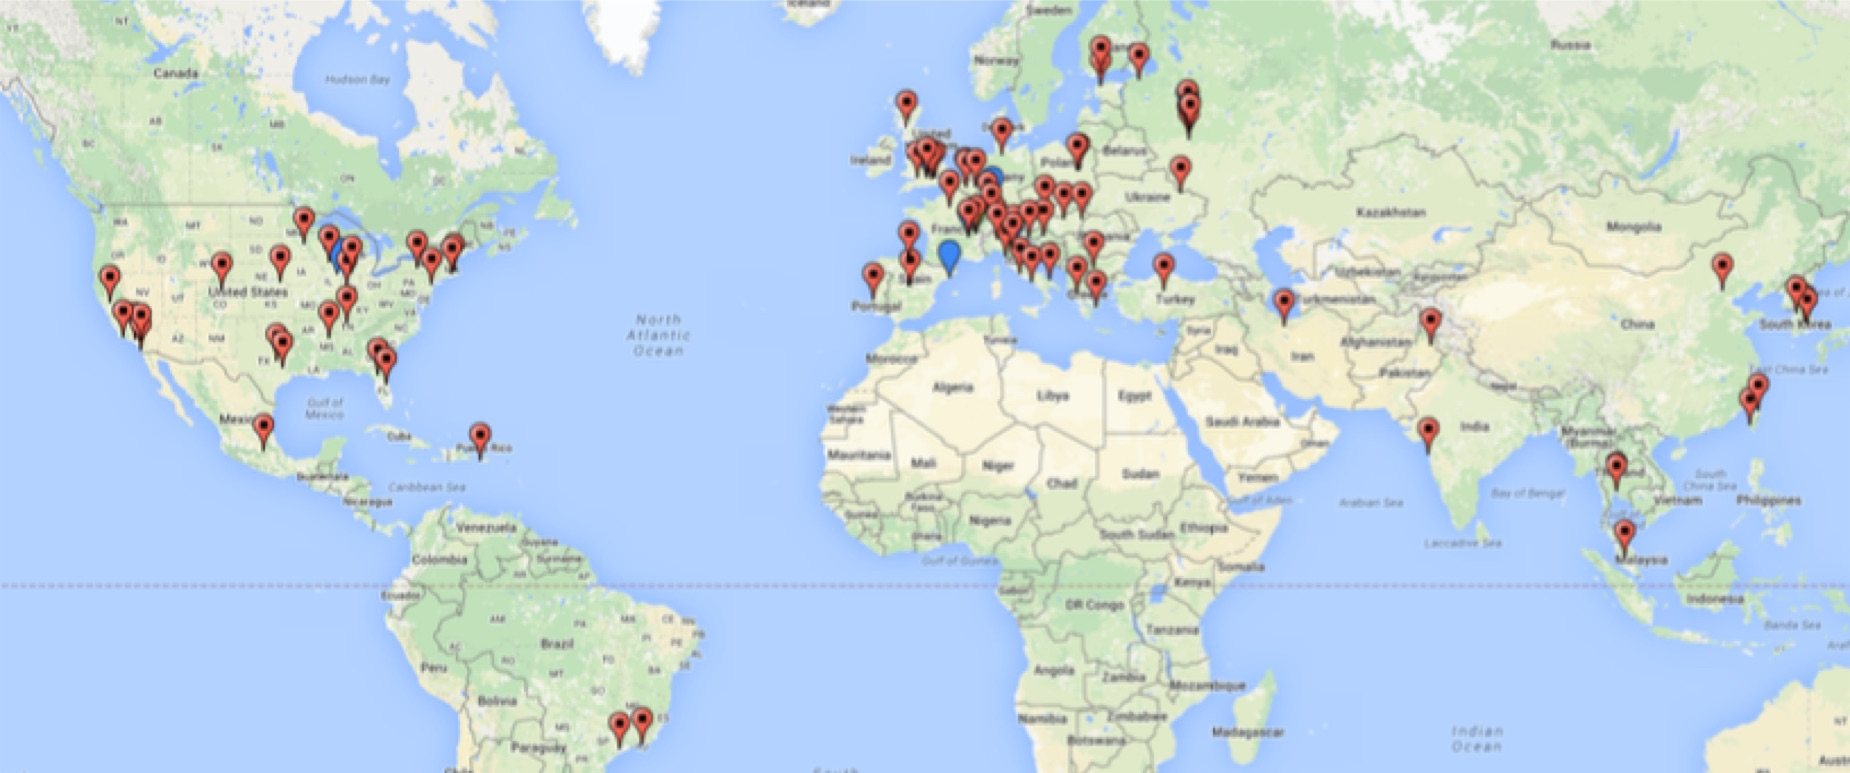
\includegraphics[width=1.0\textwidth]{images/cms-sites.jpg}
%\caption{}
%\label{fig:example2}
\end{center}
\end{figure}

\small{Over 70 sites distributed across the world}

\end{frame}



\begin{frame}
\frametitle{Data Access, Organization and Management}

\begin{itemize}
\item (See previous slide about ROOT file format)
\item Distributed computing centers requires distributed data management
\item More than just file transfers: manage retries, global placement, cleanup, archival to tape, etc.
\item Initial computing model involved static data placement in sites for access by jobs running on local compute notes
\item In recent years, we have evolved to use technologies (xrootd) allowing efficient remote (WAN) access to data: evolving global ``data federations''
\end{itemize}

\end{frame}



\begin{frame}
\frametitle{PhEDEx - Data Transfer and Placement}

\begin{figure}[htbp]
\begin{center}
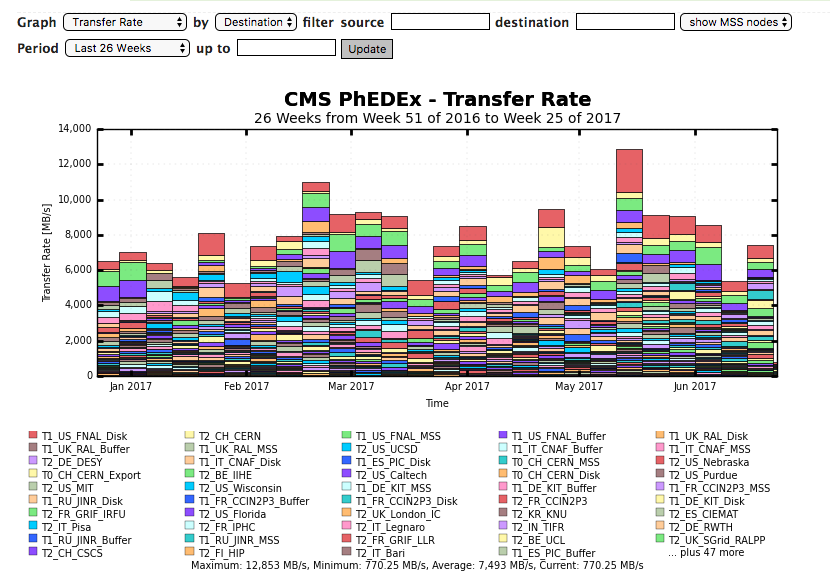
\includegraphics[width=0.85\textwidth]{images/phedex-transfers-2017-2.png}
%\caption{}
%\label{fig:example2}
\end{center}
\end{figure}

%\small{Example Text}

\end{frame}



\begin{frame}
\frametitle{Distributed Computing}
\begin{itemize}
\item Computing resources are made available to the LHC experiments in a distributed fashion
\item Significant collaboration with computer science on distributed high throughput computing via the Open Science Grid (OSG)
\item \url{https://www.opensciencegrid.org/}
\item Expected evolution in the coming years: a mix of ``owned'' resources, commercial cloud resources and use of (in particular DOE) HPC resources
\item Likely this will be more ``dynamic'' than the use of only ``owned'' (dedicated) resources as in the Grid
\end{itemize}

\end{frame}



\begin{frame}
\frametitle{HepCloud (Fermilab) AWS test}

\begin{figure}[htbp]
\begin{center}
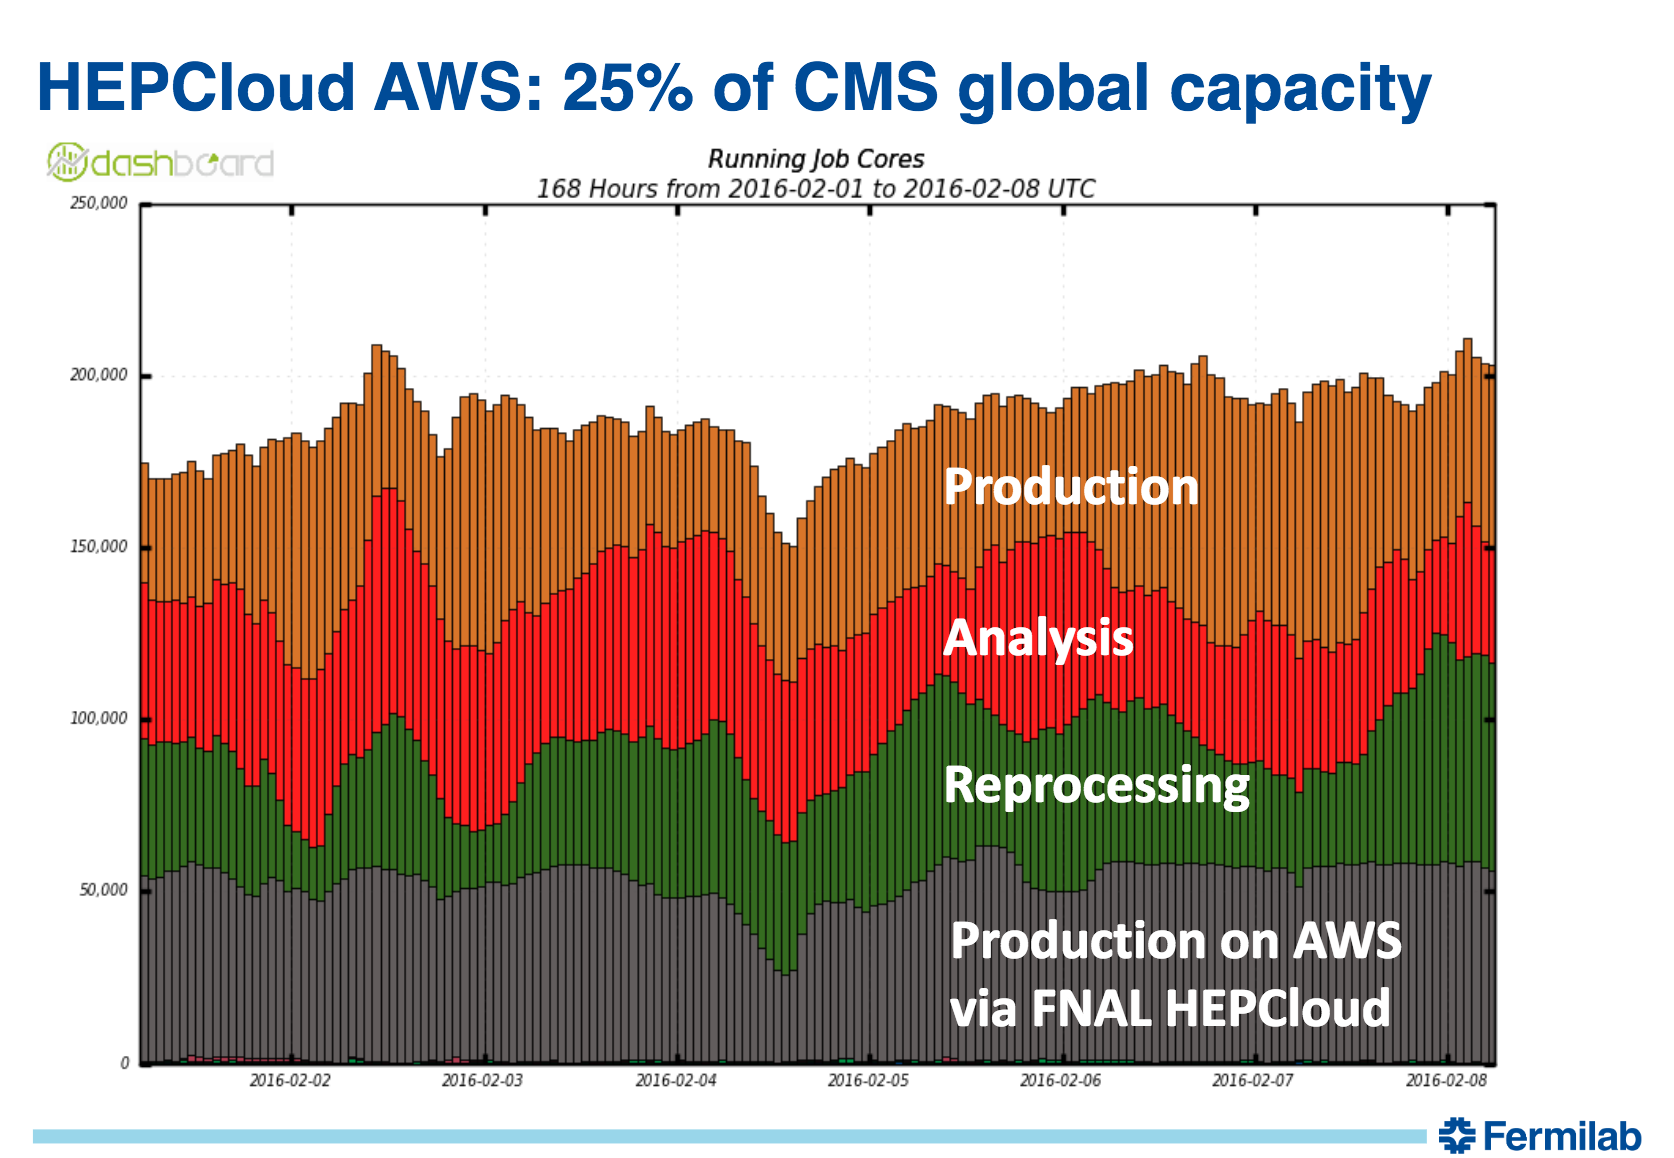
\includegraphics[width=0.7\textwidth]{images/hepcloud-aws.png}
%\caption{}
%\label{fig:example2}
\end{center}
\end{figure}

\end{frame}



\begin{frame}
\frametitle{HepCloud (Fermilab) Google Cloud test}

\begin{figure}[htbp]
\begin{center}
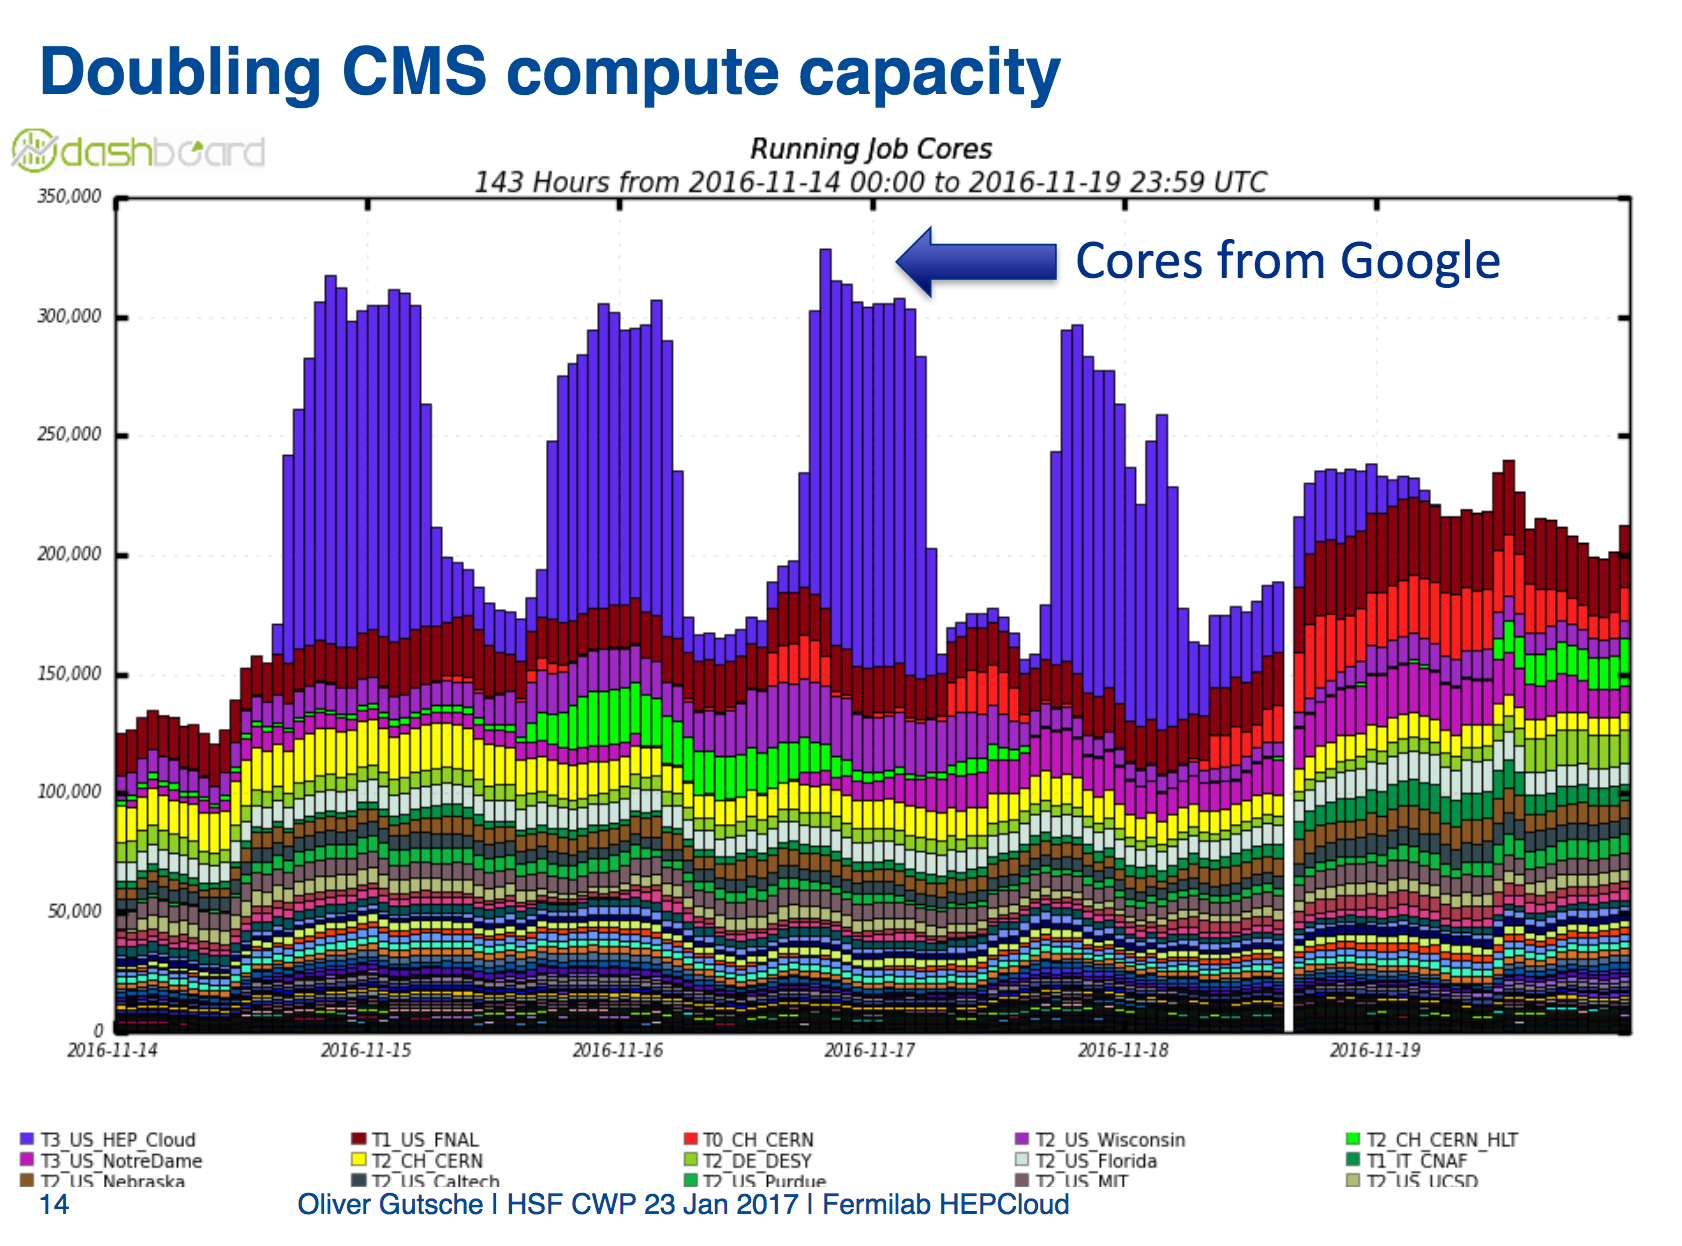
\includegraphics[width=0.7\textwidth]{images/hepcloud-google.png}
%\caption{}
%\label{fig:example2}
\end{center}
\end{figure}

\end{frame}




\begin{frame}
\frametitle{Software Trigger/Filter}

\begin{figure}[htbp]
\begin{center}
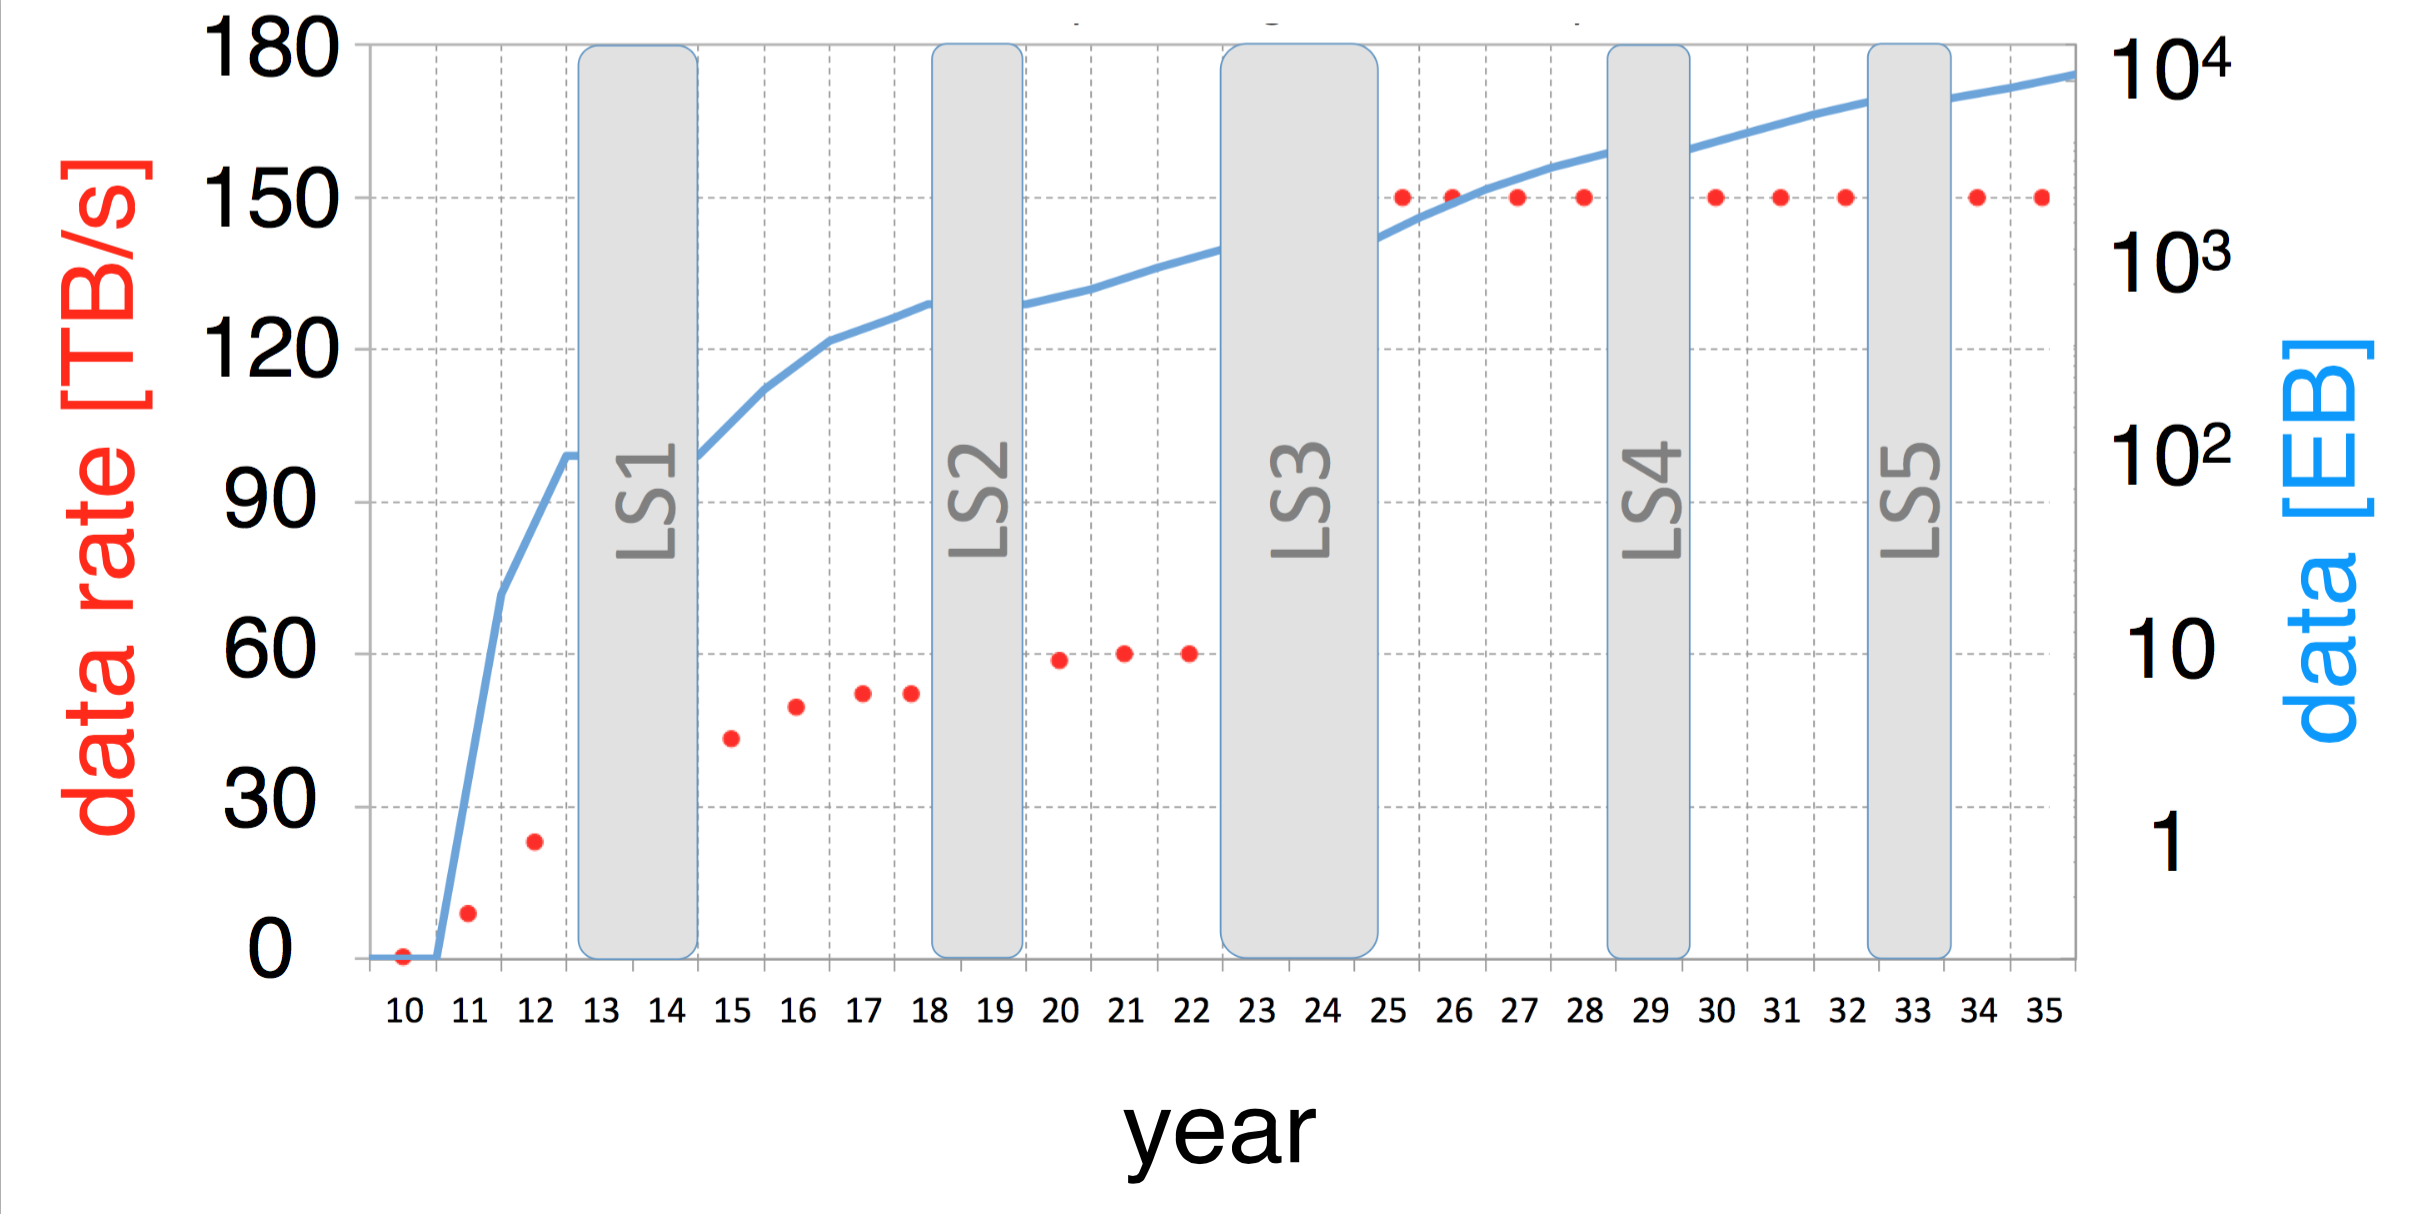
\includegraphics[width=0.8\textwidth]{images/lhc-big-data-plot.png}
%\caption{}
%\label{fig:example2}
\end{center}
\end{figure}

\small{Data ingestion rates and integral for CMS for High Level Trigger}

\end{frame}




% Collaborations
\begin{frame}
\frametitle{Particle Physics Experiments - Project Size}

\begin{figure}[htbp]
\begin{center}
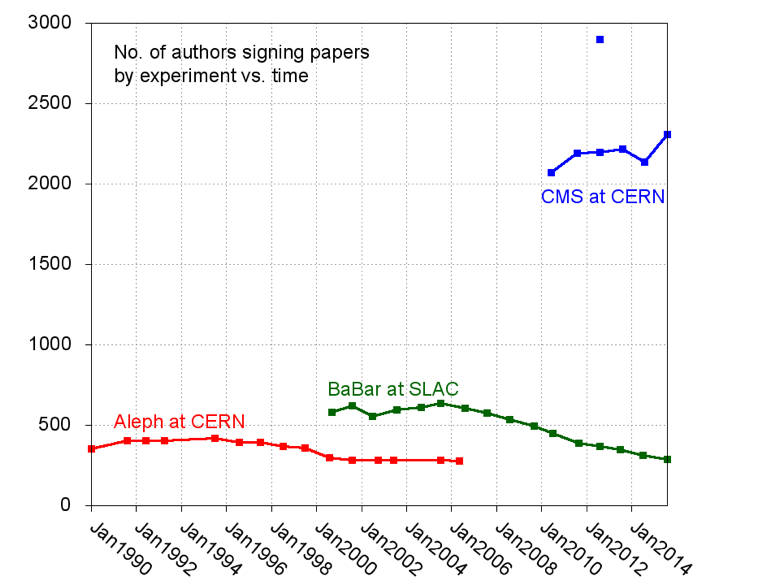
\includegraphics[width=0.8\textwidth]{images/authors-aleph-babar-cms-by-time.png}
%\caption{}
%\label{fig:example2}
\end{center}
\end{figure}

%\small{Example Text}

\end{frame}



\begin{frame}
\frametitle{BaBar collaboration - Summer 2000}

\begin{figure}[htbp]
\begin{center}
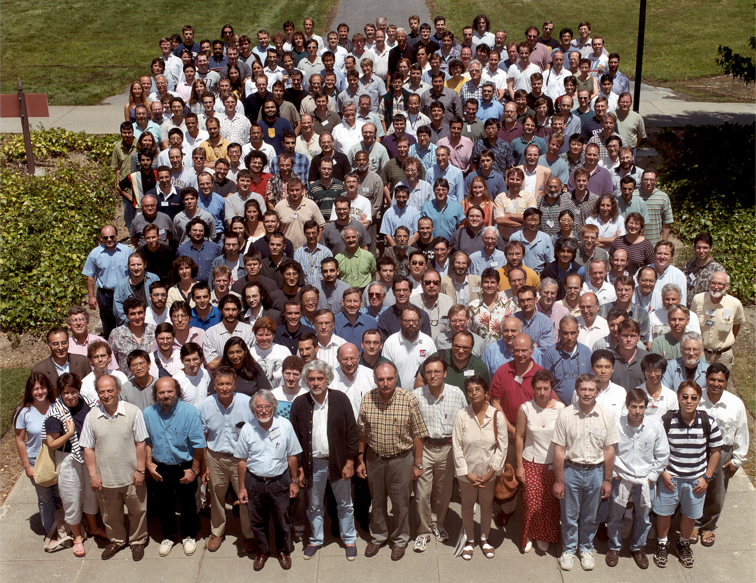
\includegraphics[width=0.7\textwidth]{images/babar-summer-2000.png}
%\caption{}
%\label{fig:example2}
\end{center}
\end{figure}

%\small{Example Text}

\end{frame}



%\begin{frame}
\frametitle{BaBar collaboration - Summer 2002}

\begin{figure}[htbp]
\begin{center}
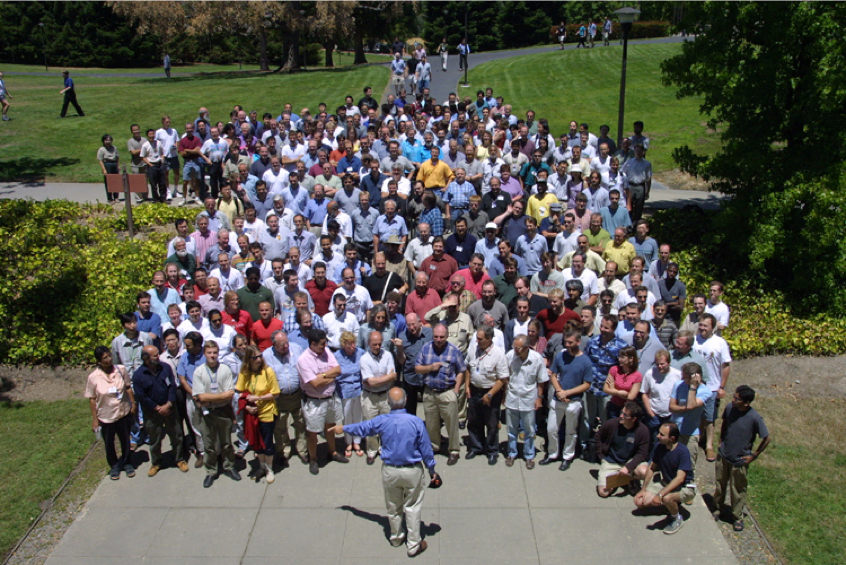
\includegraphics[width=0.7\textwidth]{images/babar-summer-2002.png}
%\caption{}
%\label{fig:example2}
\end{center}
\end{figure}

%\small{Example Text}

\end{frame}



\begin{frame}
\frametitle{CMS Collaboration - Summer 2013}

\begin{figure}[htbp]
\begin{center}
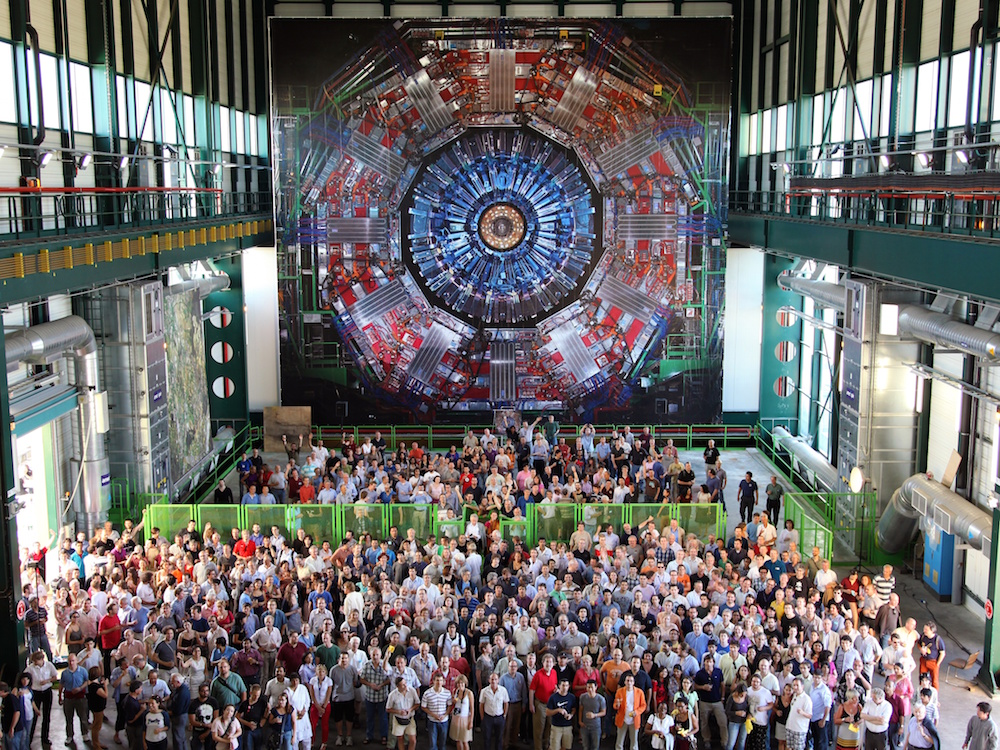
\includegraphics[width=0.8\textwidth]{images/cms-collaboration-2013-small.jpeg}
%\caption{}
%\label{fig:example2}
\end{center}
\end{figure}

\end{frame}



\begin{frame}
\frametitle{Software Process}

\begin{figure}[htbp]
\begin{center}
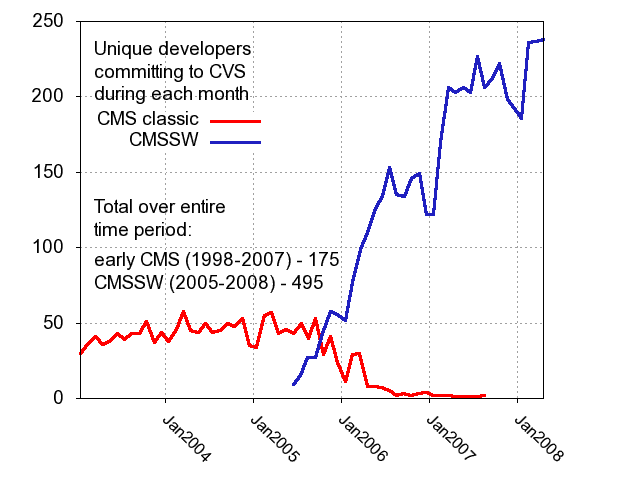
\includegraphics[width=0.8\textwidth]{images/cmssw_dev_per_month.png}
%\caption{}
%\label{fig:example2}
\end{center}
\end{figure}

\end{frame}



\begin{frame}
\frametitle{Software Process}

\begin{figure}[htbp]
\begin{center}
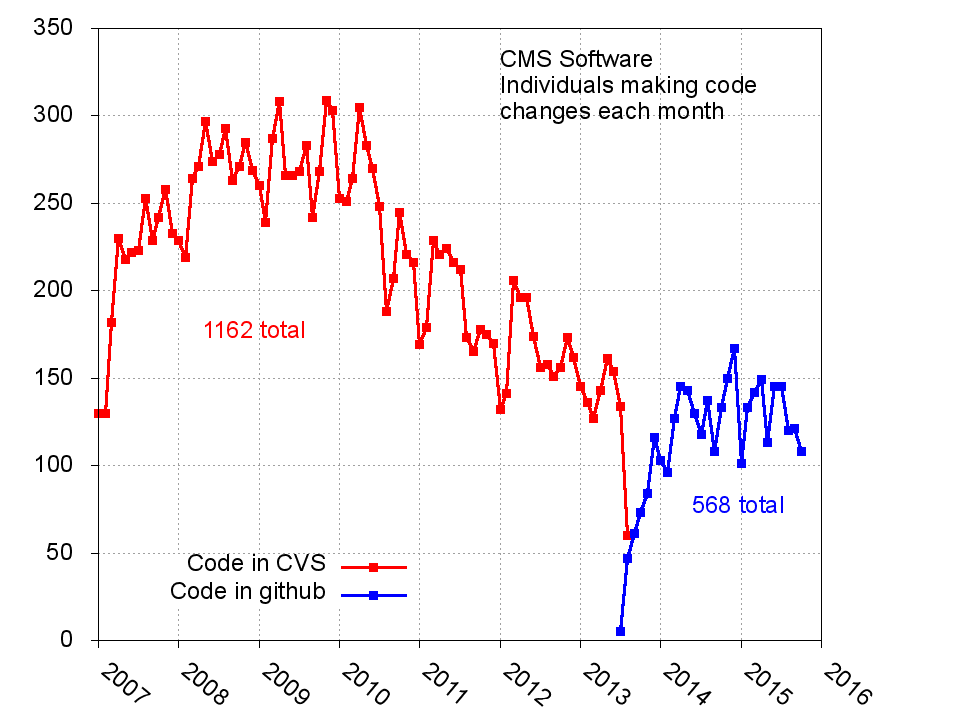
\includegraphics[width=0.8\textwidth]{images/cmssw-authors-per-month.png}
%\caption{}
%\label{fig:example2}
\end{center}
\end{figure}

\end{frame}



\begin{frame}
\frametitle{BaBar experiment - code base vs time}

\begin{figure}[htbp]
\begin{center}
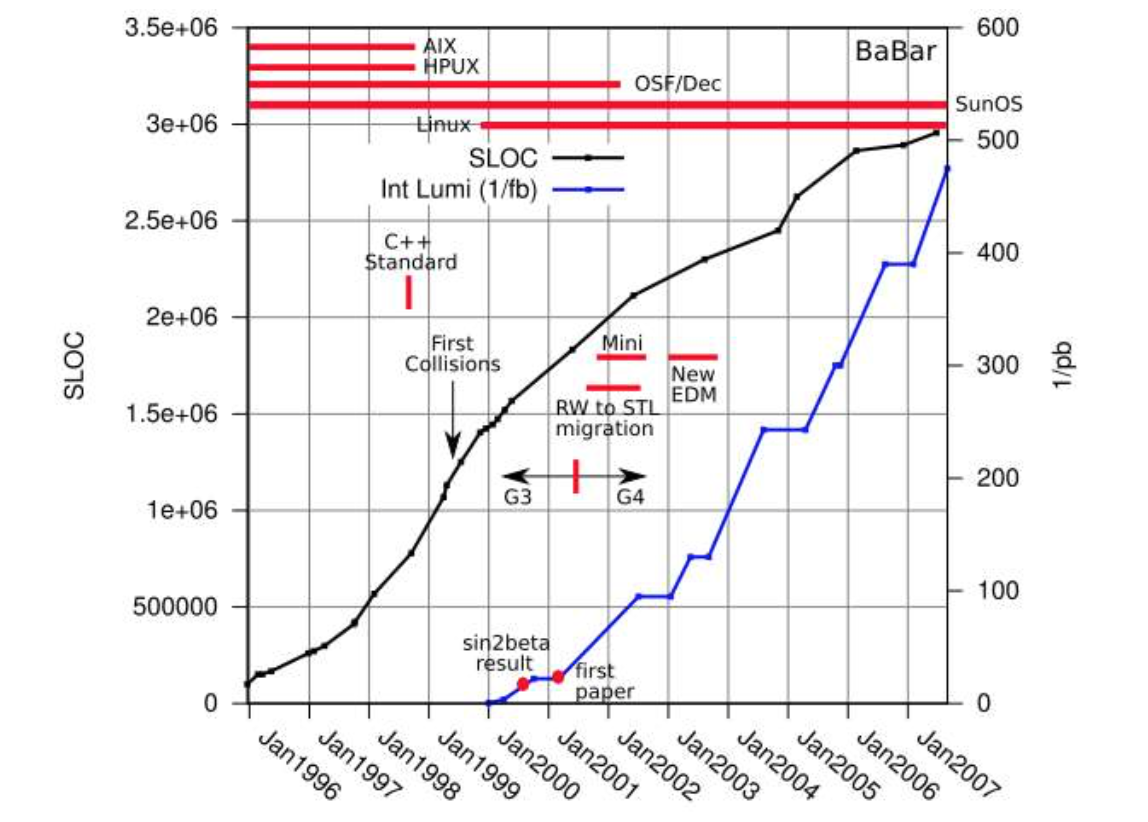
\includegraphics[width=0.9\textwidth]{images/babar-sloc-vs-time.png}
%\caption{}
%\label{fig:example2}
\end{center}
\end{figure}

\begin{center}
\small{The BaBar experiment ran from 1999 until 2008}
\end{center}

\end{frame}



\begin{frame}
%\frametitle{BaBar Experiment - ran from 1999 until 2008}
\frametitle{BaBar Experiment - Software Life Cycle}

\begin{figure}[htbp]
\begin{center}
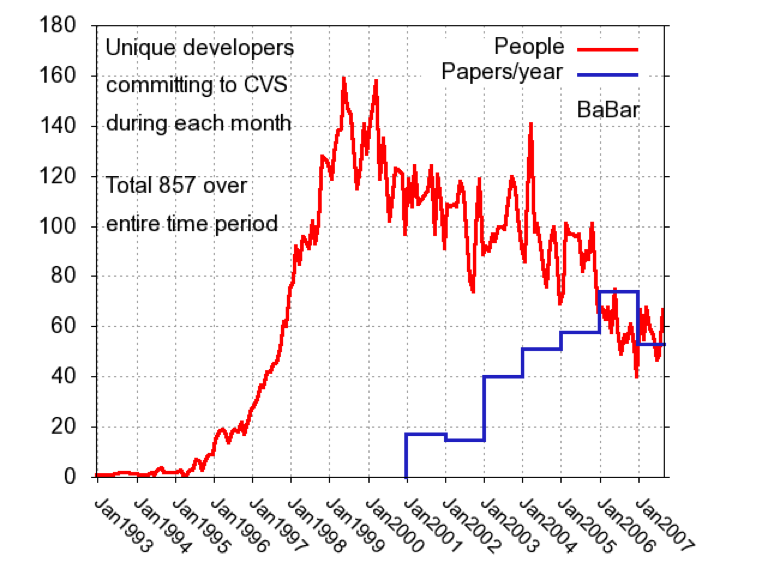
\includegraphics[width=0.7\textwidth]{images/babar-developers-per-month.png}
%\caption{}
%\label{fig:example2}
\end{center}
\end{figure}

\begin{center}
\small{Experiment ran from 1999 until 2008}
\end{center}

\end{frame}




%Challenges
\begin{frame}
\frametitle{Plans for upgrading the LHC and Experiment Detectors}

\begin{figure}[htbp]
\begin{center}
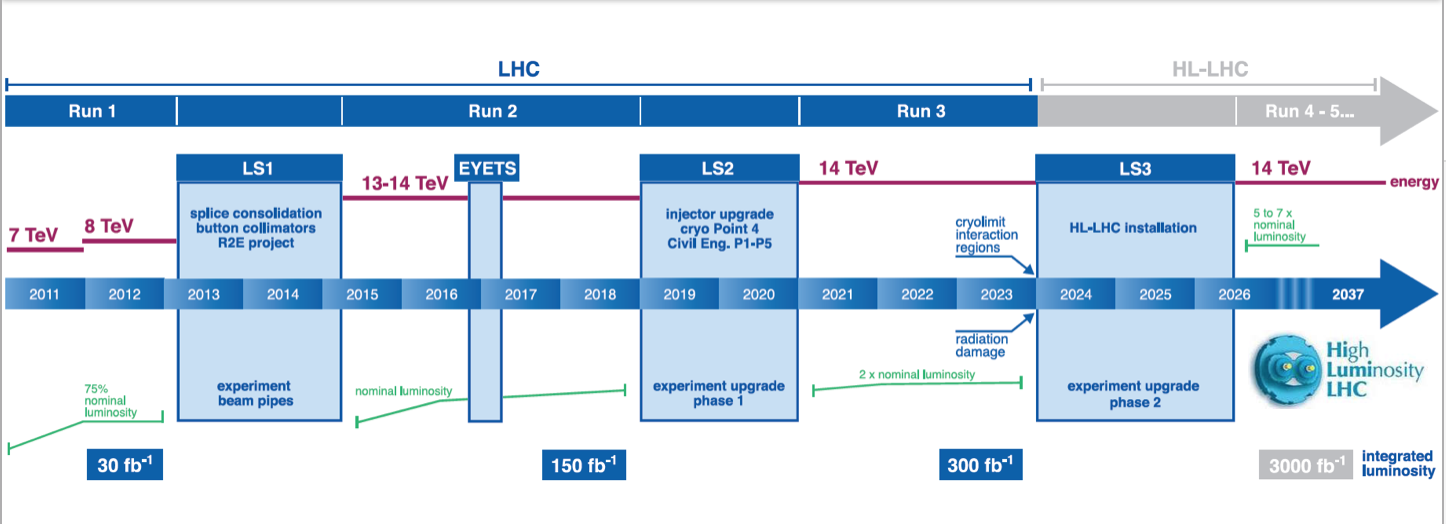
\includegraphics[width=1.0\textwidth]{images/lhc-upgrade-timeline-detail.png}
%\caption{}
%\label{fig:example2}
\end{center}
\end{figure}

\small{Major hardware upgrades to both the LHC and the detectors/experiments are planned in the ``long shutdowns''}

\end{frame}



\begin{frame}
\frametitle{CMS HL-LHC upgrades}

\begin{figure}[htbp]
\begin{center}
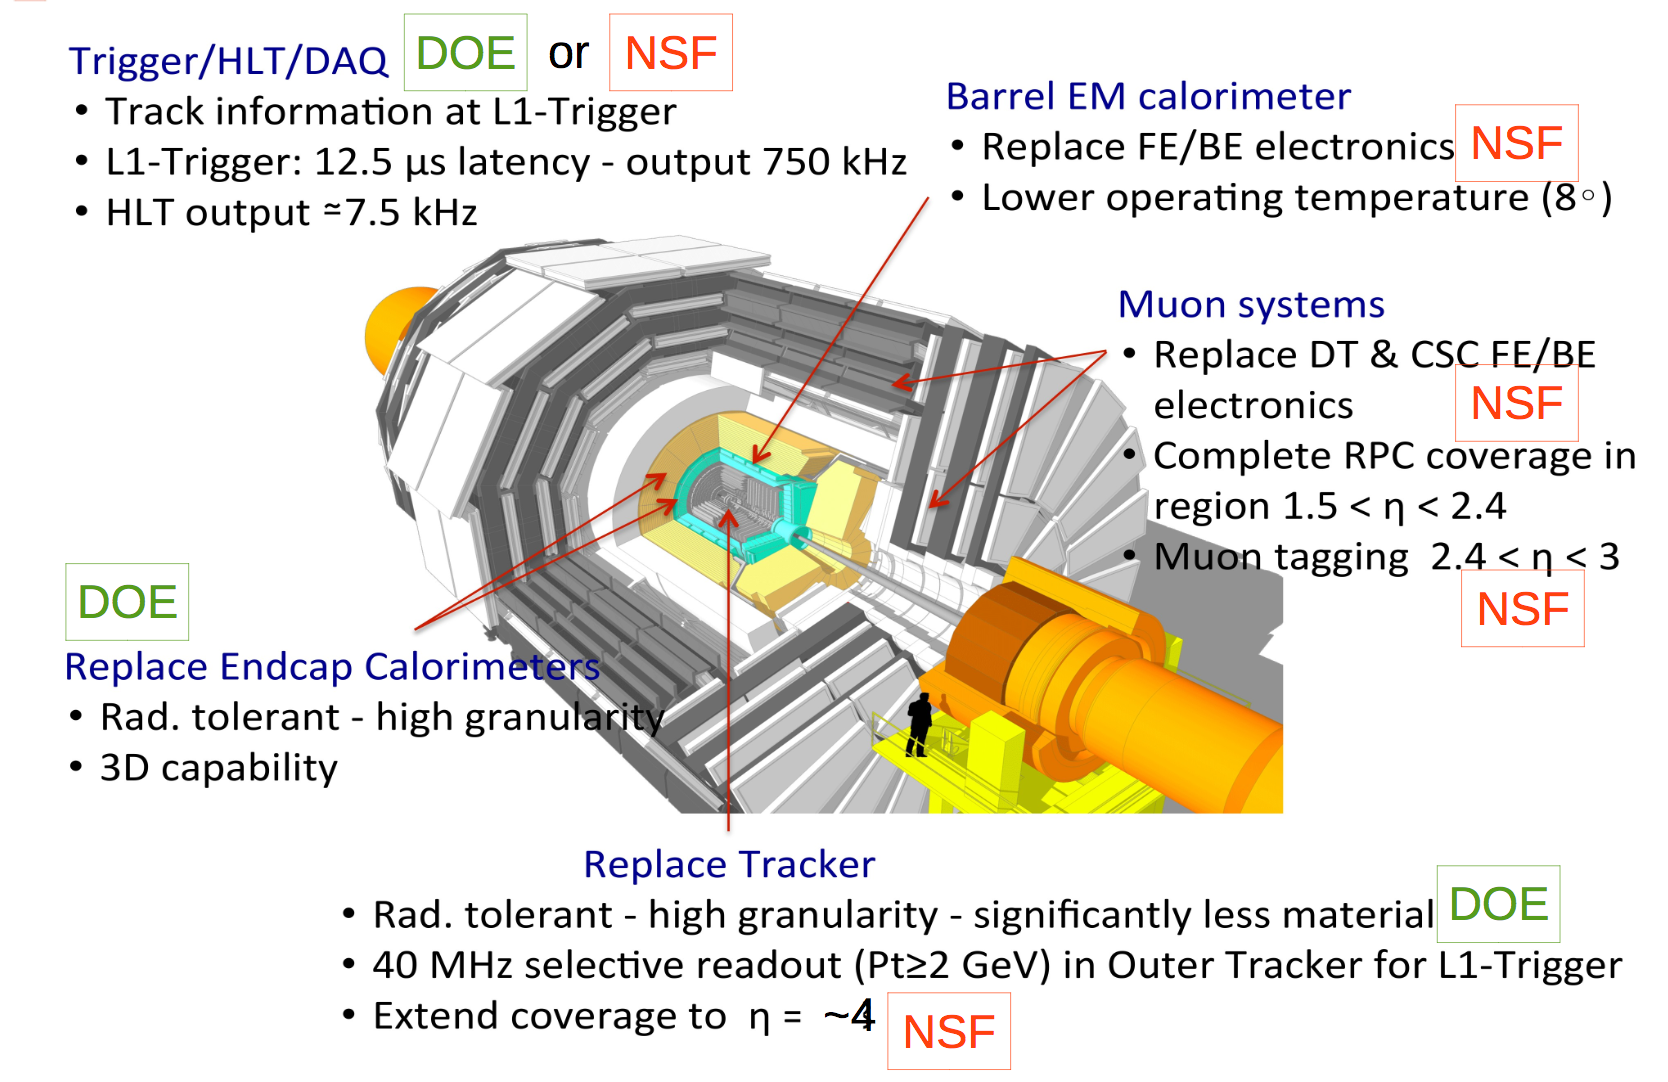
\includegraphics[width=0.9\textwidth]{images/hl-lhc-upgrade-cms-anders-ryd.png}
%\caption{}
%\label{fig:example2}
\end{center}
\end{figure}

%\small{Example Text}

\end{frame}



%\begin{frame}
\frametitle{Large Hadron Collider Notes}

\begin{itemize}
\item (Geographically) Distributed High Throughput Computing
\item Currently aggregating resources from US Universities (NSF and local
compute), DOE labs (FNAL, BNL, SLAC), and international 
\item Going forward we expect we will need to aggregate over ``owned'' resources, DOE HPC resources (e.g. NERSC, ANL, ORNL) {\it and} commercial clouds
\item FNAL HEPCloud: demonstrated at-scale use with AWS and Google Cloud 
\item TIFR Mumbai currently testing with Microsoft Azure
\item DOE (HTC on) HPC: Ongoing work to use Mira (ANL) and Edison/Cori (NERSC)
\end{itemize}

\end{frame}



\begin{frame}
\frametitle{LHC Luminosity Evolution}

\begin{figure}[htbp]
\begin{center}
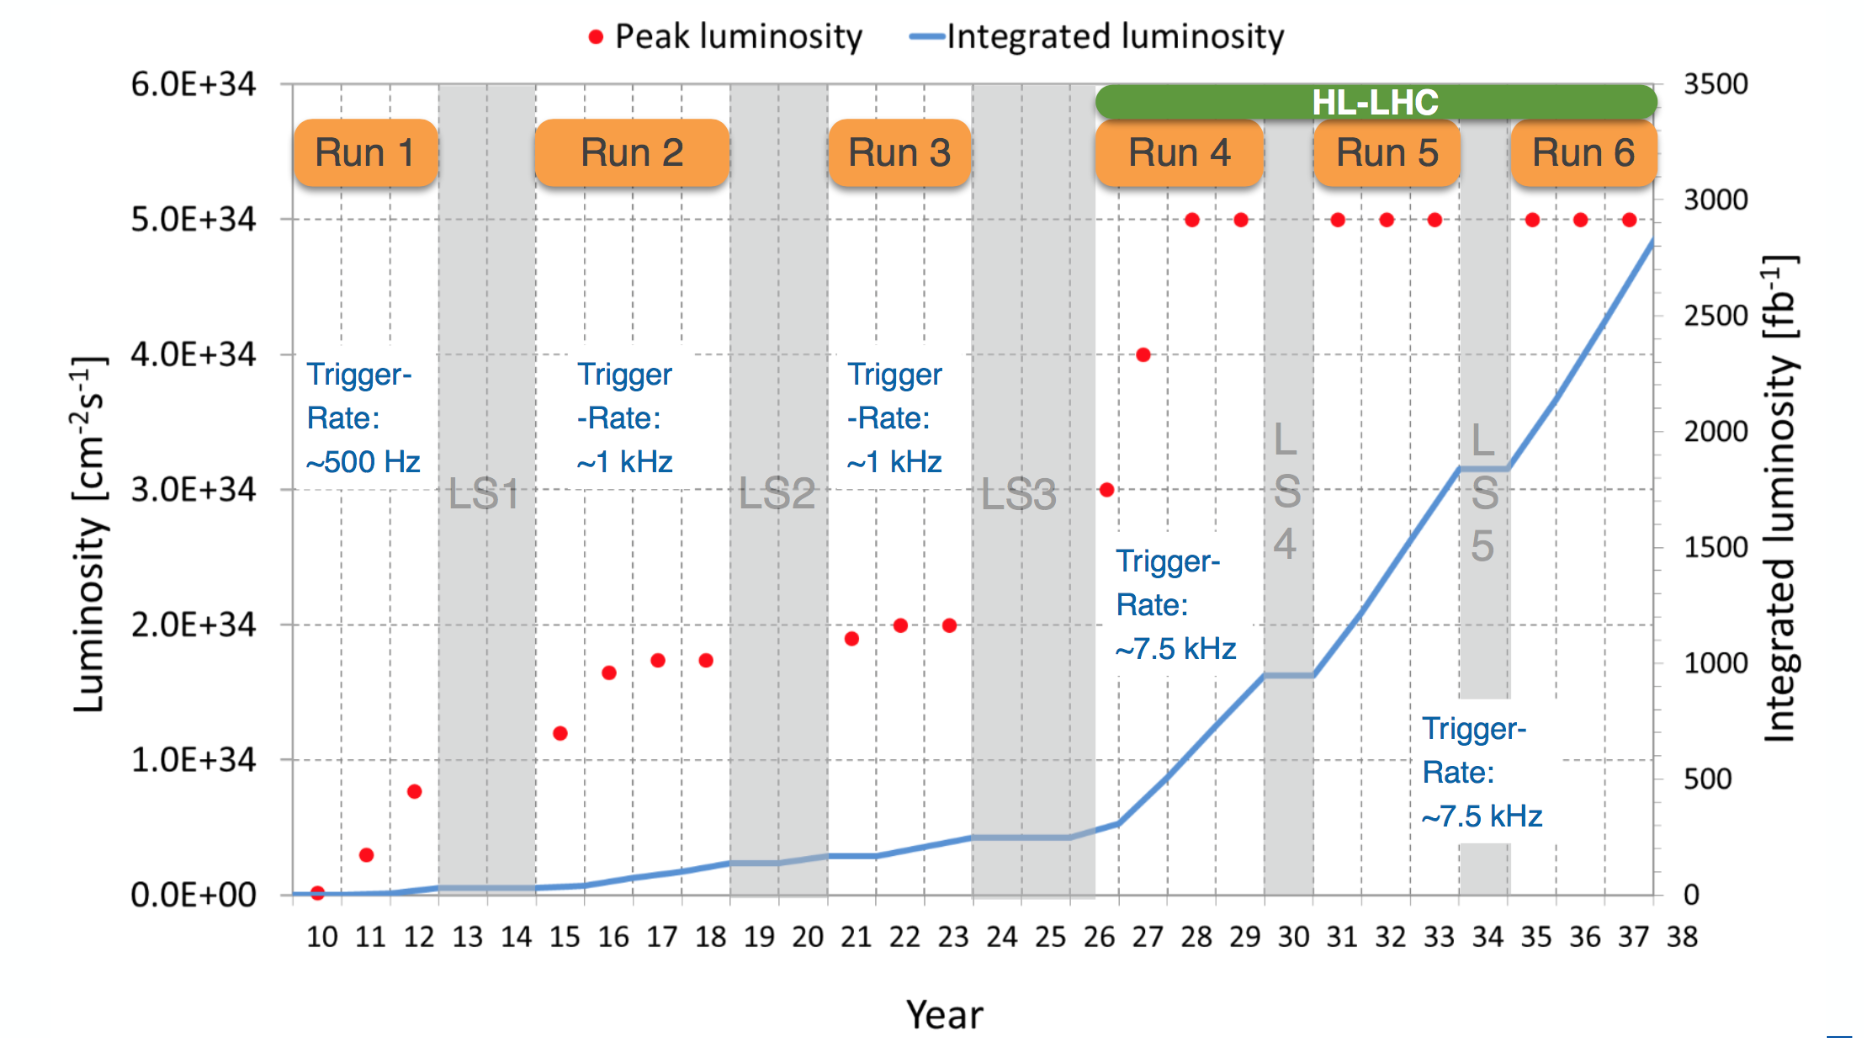
\includegraphics[width=0.9\textwidth]{images/lhc-lumi-evolution.png}
%\caption{}
%\label{fig:example2}
\end{center}
\end{figure}

%\small{Example Text}

\end{frame}



\begin{frame}
\frametitle{Estimates of Resource Needs for HL-LHC (WLCG)}

\begin{figure}[htbp]
\begin{center}
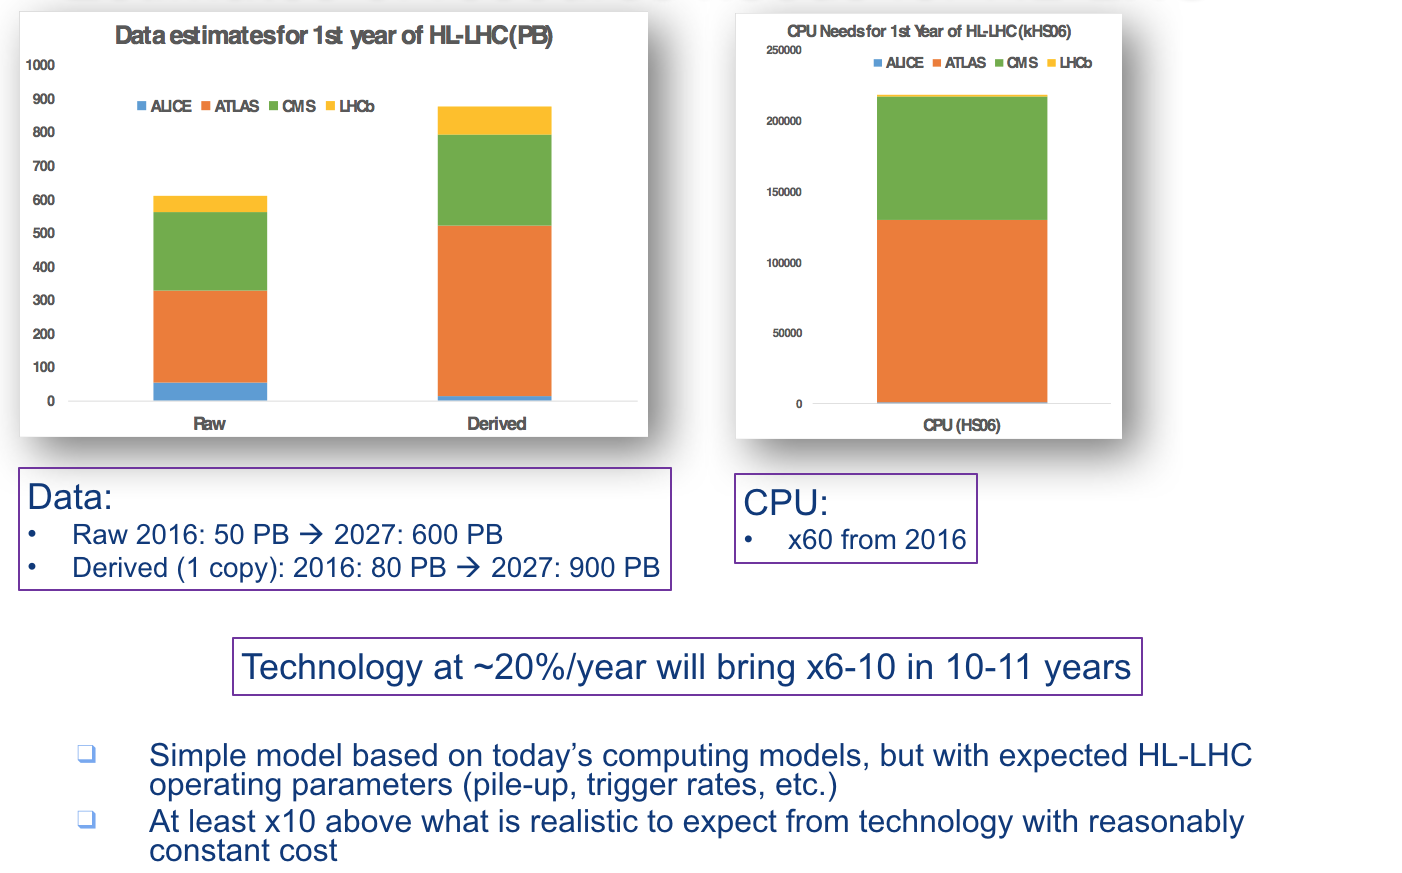
\includegraphics[width=0.95\textwidth]{images/20161008-wlcg-intro-ian-bird-slide-10.png}
\end{center}
\end{figure}

%\begin{center}
%\small{(Slide from WLCG Workshop Intro, Ian Bird, 8 Oct, 2016)}
%\end{center}

\end{frame}



\begin{frame}
\frametitle{A Software ``Upgrade'' for HL-LHC and 2020s HEP?}

Looking forward to the next 10 years, we see a number of challenges for HEP software and computing:

\begin{itemize}
\item {\bf Performance/cost:} Estimates of computing needs run faster than Moore's Law by factors of o(10)
\item {\bf Technology/Market evolution:} the return of heterogeneity; technology change will also make it challenging to exploit Moore's Law without software evolution.
\item {\bf Scale:} The HL-LHC will integrate 100 times the current data, with significantly increased data (pileup) and detector complexity.
\item {\bf Sustainability:} Most of the current software, which defines our capabilities, was designed 15-20 years ago: there are many software sustainability challenges.
\end{itemize}

\end{frame}



\begin{frame}
\frametitle{Processor evolution and software impact}

\begin{columns}[T] % align columns

\begin{column}{.48\textwidth}
\begin{figure}[htbp]
\begin{center}
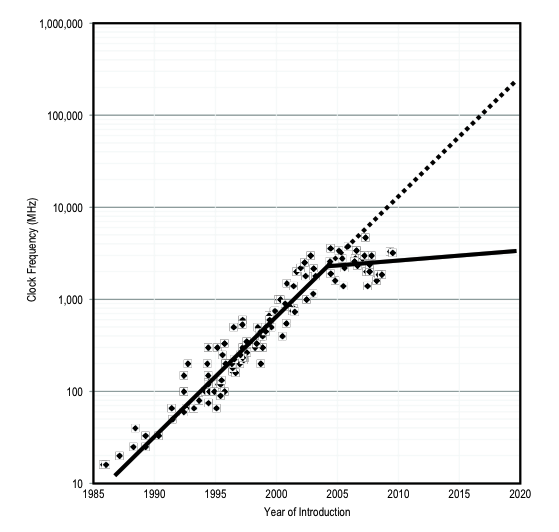
\includegraphics[width=1.0\textwidth]{images/moore2.png}
\end{center}
\end{figure}
\begin{center}
\small{Clock Frequency vs Time}
\end{center}
\end{column}%

\hfill%

\begin{column}{.48\textwidth}
\begin{itemize}
\item Single core performance has stalled, leading to multi/manycore and specialization
\item To even realize Moore's Law gains, we are pushed towards parallelization of algorithms and design for performance.
\item The software designs and implementations themselves need to evolve, not just be recompiled
\end{itemize}
\end{column}%

\end{columns}

\end{frame}



\begin{frame}
\frametitle{Back to heterogeneous systems?}

Building the worldwide distributed LHC computing grid was largely made possible by the convergence on Linux on (commodity) Intel x86 processors around the year 2000. Building the WLCG at this scale in the heterogeneous workstation era would have been quite difficult. For better or for worse, heterogeneity is returning:

\begin{itemize}
\item Diversity of computing processor architectures (general purpose cores vs specialized processors)
\item Owned vs commercial/cloud providers
\item Some pressure to use systems traditionally designed for other types of applications (e.g.\ HPC/supercomputer as opposed to HTC/high-throughput systems)
\item Possible further commoditizing market pressures (e.g. mobile)
\end{itemize}

\end{frame}



\begin{frame}
\frametitle{What is software sustainability?} 
\begin{itemize}
\item {\bf Dependent Infrastructure:} Will the infrastructure element continue to provide the same functionality in the future, even when the other parts of the infrastructure on which the element relies change?
\item {\bf Collaborative Infrastructure} Can the element be combined with other elements to meet user needs, as both the collaborative elements and the individual elements change?
\item {\bf New Users:} Is the functionality and usability of the infrastructure element clearly explained to new users? Do users have a mechanism to ask questions and to learn about the element?
\item {\bf Existing Users:} Does the infrastructure element provide the functionality that current users want? Is it modular and adaptable so that it can meet the future needs of the users?
\item {\bf Science:} Does it incorporate and implement new science and theory as they develop?
\end{itemize}

\tiny{ Katz, D.S. \& Proctor, D., (2014). A Framework for Discussing e-Research Infrastructure Sustainability. Journal of Open Research Software. 2(1), p.e13. DOI: http://doi.org/10.5334/jors.av}
\end{frame}






% 
\begin{frame}
\frametitle{HEP Software Foundation (HSF)}

\begin{columns}[T] % align columns

\begin{column}{.75\textwidth}
The HSF (http://hepsoftwarefoundation.org) was created in early 2015 as a means for organizing our community to address the software challenges of future projects such as the HL-HLC. The HSF has the following objectives: 
\end{column}%

\hfill%

\begin{column}{.20\textwidth}
\begin{figure}[htbp]
\begin{center}

\includegraphics[width=1.0\textwidth]{images/hsf_logo_angled.png}
\end{center}
\end{figure}
\end{column}%

\end{columns}

\vskip 0.1in

\begin{itemize}
\item Catalyze new common projects
\item Promote commonality and collaboration in new developments to make the most of limited resources
\item Provide a framework for attracting effort and support to S\&C common projects (new resources!)
\item Provide a structure to set priorities and goals for the work
\end{itemize}

%An initial set of collaborative activities have begun (see recent HSF workshop 
%at LAL-Orsay). 


\end{frame}



\begin{frame}
\frametitle{HEP Software Foundation} 

\begin{figure}[htbp]
\begin{center}
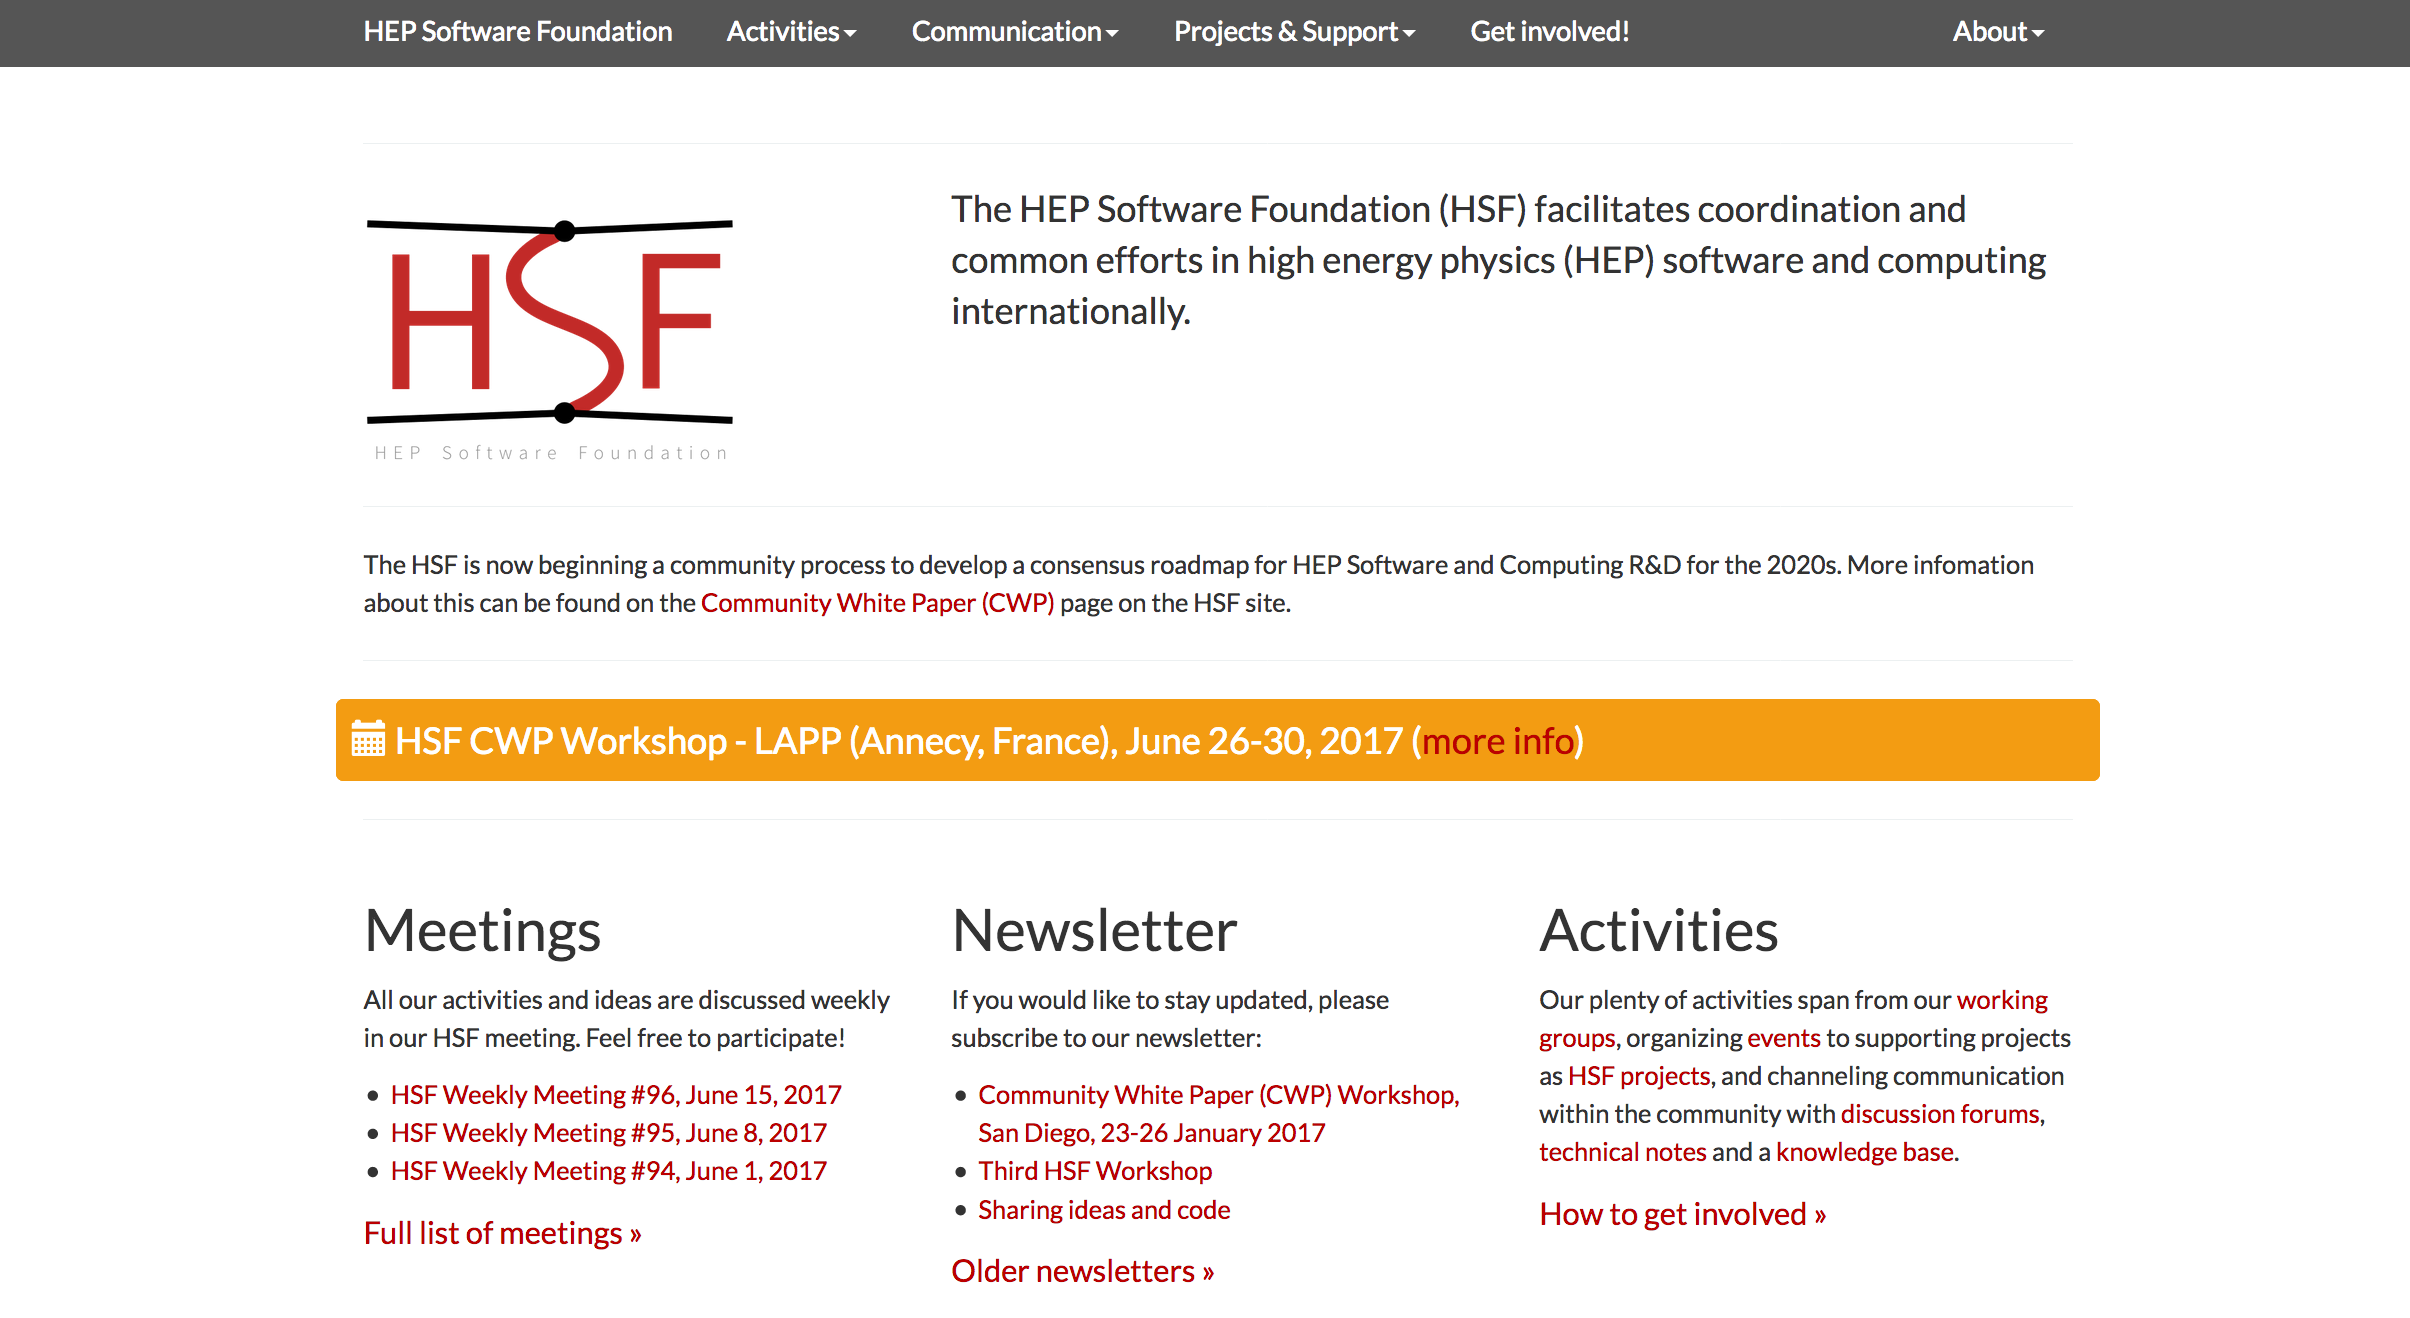
\includegraphics[width=1.0\textwidth]{images/20170621-hsf-website.png}
%\caption{}
%\label{fig:example2}
\end{center}
\end{figure}

\small{\url{http://hepsoftwarefoundation.org/}}

\end{frame}



\begin{frame}
\frametitle{Community White Paper (CWP) Goals}

To prepare for the challenges of the High Luminosity Large Hadron Collider (HL-LHC), the CWP should identify and prioritize the software research and development investments required:

\begin{enumerate}
\item to achieve improvements in software efficiency, scalability and performance and to make use of the advances in CPU, storage and network technologies
\item to enable new approaches to computing and software that could radically extend the physics reach of the detectors
\item to ensure the long term sustainability of the software through the lifetime of the HL-LHC
\end{enumerate}

\end{frame}



\begin{frame}
\frametitle{S2I2-HEP Conceptualization Project}

\begin{figure}[htbp]
\begin{center}
\includegraphics[width=1.0\textwidth]{images/20170621-s2i2-hep-webpage.png}
%\caption{}
%\label{fig:example2}
\end{center}
\end{figure}

\small{\url{http://s2i2-hep.org/}}

\end{frame}



\begin{frame}
\frametitle{S2I2 HEP Events}

\begin{columns}[T] % align columns

\begin{column}{.50\textwidth}
\begin{figure}[htbp]
\begin{center}
\includegraphics[width=1.0\textwidth]{images/s2i2-hep-events-1.png}
%\caption{}
%\label{fig:example2}
\end{center}
\end{figure}
\end{column}%

\begin{column}{.50\textwidth}
\begin{figure}[htbp]
\begin{center}
\includegraphics[width=1.0\textwidth]{images/s2i2-hep-events-2.png}
%\caption{}
%\label{fig:example2}
\end{center}
\end{figure}
\end{column}%




\end{columns}

%\small{Example Text}

\end{frame}



\begin{frame}
\frametitle{S2I2 HEP Workshops with Computer Scientists}

\begin{figure}[htbp]
\begin{center}
\includegraphics[width=0.65\textwidth]{images/20161208-S2I2-HEP-CS-UIUC-group-photo.jpeg}
%\caption{}
%\label{fig:example2}
\end{center}
\end{figure}

\small{UIUC, 7-9 Dec, 2016, \url{https://indico.cern.ch/event/575443/}}

\begin{figure}[htbp]
\begin{center}
\includegraphics[width=0.55\textwidth]{images/20170502-S2I2-HEP-CS-Princeton-group-photo.jpeg}
%\caption{}
%\label{fig:example2}
\end{center}
\end{figure}

\small{Princeton, 1-3 May, 2017, \url{https://indico.cern.ch/event/622920/}}


\end{frame}



\begin{frame}
\frametitle{S2I2 HEP Workshops with Computer Scientists}

\begin{itemize}
\item HEP offers at-scale production-capable systems for a variety of CS research topics: scalable systems, data management, paralel
\item ``industry scale, academic openness''
\item Developing collaborations requires HEP to recognize that CS research interests differ from HEP research interests.
\item Communication gaps exist: not only jargon, but also in simply formulating the problem to solve. Significant assumptions and/or incomplete problem descriptions. HEP people often describe the problem in terms of the solution we have at the moment.
\item Recognition that building common terminology and involving CS researchers earlier in the process will be beneficial.
\end{itemize}

\end{frame}



\begin{frame}
\frametitle{Software Sustainability Institute (UK)}

\begin{figure}[htbp]
\begin{center}
\includegraphics[width=0.75\textwidth]{images/ssi-uk-activities.png}
%\caption{}
%\label{fig:example2}
\end{center}
\end{figure}

\small{(Slide from Neil Chue Hong, SSI)}

\end{frame}



\begin{frame}
\frametitle{The DIANA/HEP project}

\begin{itemize}
\item Data Intensive ANAlysis for High Energy Physics (DIANA/HEP)
\item The primary goal of DIANA/HEP is to develop state-of-the-art tools for experiments which acquire, reduce, and analyze petabytes of data.
\item DIANA is not a piece of software itself, but a collaborative project to improve and extend analysis tools as sustainable infrastructure for the community.
\item Funded by NSF ``Software Infrastructure for Sustained Innovation'' (SI2) program
\item 4-year project, 6-7FTE total
\item Princeton, NYU, UCincinnati, U.Nebraska-Lincoln
\item The PIs are involved in Atlas, CMS and LHCb
\end{itemize}

\end{frame}



\begin{frame}
\frametitle{The DIANA/HEP Project (http://diana-hep.org)}

\begin{figure}[htbp]
\begin{center}
\includegraphics[width=1.0\textwidth]{images/20160610-diana-hep-banner.png}
\end{center}
\end{figure}

\small{The DIANA/HEP project focuses on improving performance, interoperability, and collaborative tools through modifications and additions to ROOT and other packages broadly used by the HEP community.}
\vskip 0.15in
\small{Website: \url{http://diana-hep.org}}
\vskip 0.05in
\small{Google group: \url{https://groups.google.com/forum/\#!forum/diana-hep}}
\vskip 0.05in
\small{Github: \url{https://github.com/diana-hep}}

\end{frame}



\begin{frame}
\frametitle{DIANA/HEP team}

\begin{figure}[htbp]
\begin{center}
\includegraphics[width=0.8\textwidth]{images/20170110-diana-team.png}
%\caption{}
%\label{fig:example2}
\end{center}
\end{figure}

\end{frame}



\begin{frame}
\frametitle{DIANA/HEP collaborators}

\begin{figure}[htbp]
\begin{center}
\includegraphics[width=0.9\textwidth]{images/20170110-diana-collaborators.png}
%\caption{}
%\label{fig:example2}
\end{center}
\end{figure}

\end{frame}





\begin{frame}
\frametitle{Summary}
\begin{itemize}
\item Modern data science is now realizing that 80\% of the effort is in collecting, cleaning and organizing data and only a small fraction is in actual analysis.
\item The intellectual products of these activities are captured in software. This is the true cyberinfrastructure.
\item High Energy Physics has been building and evolving tools for the full range of activities over decades and is now working towards building the tools for the next 20 years of activities
\item Similar statements can be made about the human organizational and collaborative structures around these activities
\item Sustainability and evolution of software as a critical research infrastructure mostly involves work on these human structures in the system
\end{itemize}

\end{frame}




%\begin{frame}
\frametitle{}

\begin{center}
    Backup slides
\end{center}

\end{frame}




\end{document}
